\documentclass[russian, 12pt]{article}

\usepackage[utf8x]{inputenc}
\usepackage[T2A]{fontenc}
\usepackage[russian]{babel}
\usepackage{amsfonts}
\usepackage{amssymb,amsmath,color}
\usepackage{wrapfig}
\usepackage{graphicx}
\usepackage{indentfirst}
\usepackage{commath}
\usepackage{multicol}
\usepackage{geometry}
\usepackage{textcomp}
\usepackage{esint}
\usepackage{mathrsfs}
\usepackage{float}
\usepackage{cancel}
\usepackage{empheq}
\usepackage{xr}
\usepackage{array}
\usepackage{tabu}
\usepackage{setspace}


\DeclareGraphicsExtensions{.pdf,.png,.jpg}
\graphicspath{}
\setcounter{page}{1}
\begin{document}

\section{Основные понятия}
\subsection{Событие. Вероятность события}
При рассмотрении опытов в которых могут быть различные исходы, результаты опытов будем называть событиями. Отличаем составные (разложимые) и элементарные (неразложимые) события.\\
\textbf{Пример} \\Выпало 6 очков при броске двух игральных костей -- составное разложение на (1, 5) или (2,4) или (3,3) или (4,2) или (5,1). \\
О том, что мы понимаем под элементарным событием надо предварительно условиться. Это неопределяемое понятие (как точка в геометрии). Они определяют идеализированный опыт. По определению, каждый  неразложимый исход идеализированного опыта представляется одним и только одним элементарным событием. Совокупность всеъ элементарных событий называется пространством элементарных событий  ($\sigma$). Элементарное событие -- точки этого пространства. Событие -- множество точек.\\
Совокупность точек представляет все те исходы, при которых происходит событие $A$, полностью описывают это событие. Любое множество точек А нашего пространства можно назвать событием; оно происходит или нет в зависимости от того, принадлежит или нет множеству $A$ точка, представляющая исходный опыт.\\
\textbf{Пример}\\ Число курящих среди 100 человек. Пространство элементарных событий -- множество чисел 0, 1, 2,  . . . 100.\\
\textit{\textbf{Определение}}\\Невозможное событие -- это событие, которое в результате данного опыта не может произойти. Обозначим его $\emptyset$. То есть, запись $A$ = $\emptyset$ означает, что $A$ не содержит элементарных событий.\\
\textbf{Пример}\\Рассмотрим систему, состоящую из 6 атомов H. Выбираем один атом.\\
\textit{\textbf{Определение}} \\Достоверное событие -- то, которое в результате опыта  обязательно произойдет. То есть $A$ = ($\sigma$).\\
\textbf{Пример}\\Достоверное событие -- выпадение $\leq$ 6 очков при броске одной игральной кости.\\
\textit{\textbf{Определение}}\\ Событие, состоящее из всех точек, не содержащих событие А, называется событием противоположным А и обозначается $\overline{A}$.\\
$\overline{\sigma}$ = $\emptyset$.\\
$A$ -- выпадение орла, $\overline{A}$ -- решки.\\
\textit{\textbf{Определение}}\\ Суммой (объединением)  $A$ + $B$ $(A \cup B)$ событий $A$ и $B$ назовем событие, которое состоит в том, что имеет место или $A$, или $B$, или (и $A$, и $B$). То есть это обьединение множеств точек $A$ и $B$.\\
%начало страницы 2
\textit{\textbf{Определение}}\\Произведением (пересечением) $A$ $\cdot$ $B$ $(A \cap B)$ событий $A$ и $B$ называется событие, которое состоит в том, что имеет место и $A$ и $B$(одновременно) -- пересечение множества точек $A$ и $B$.\\
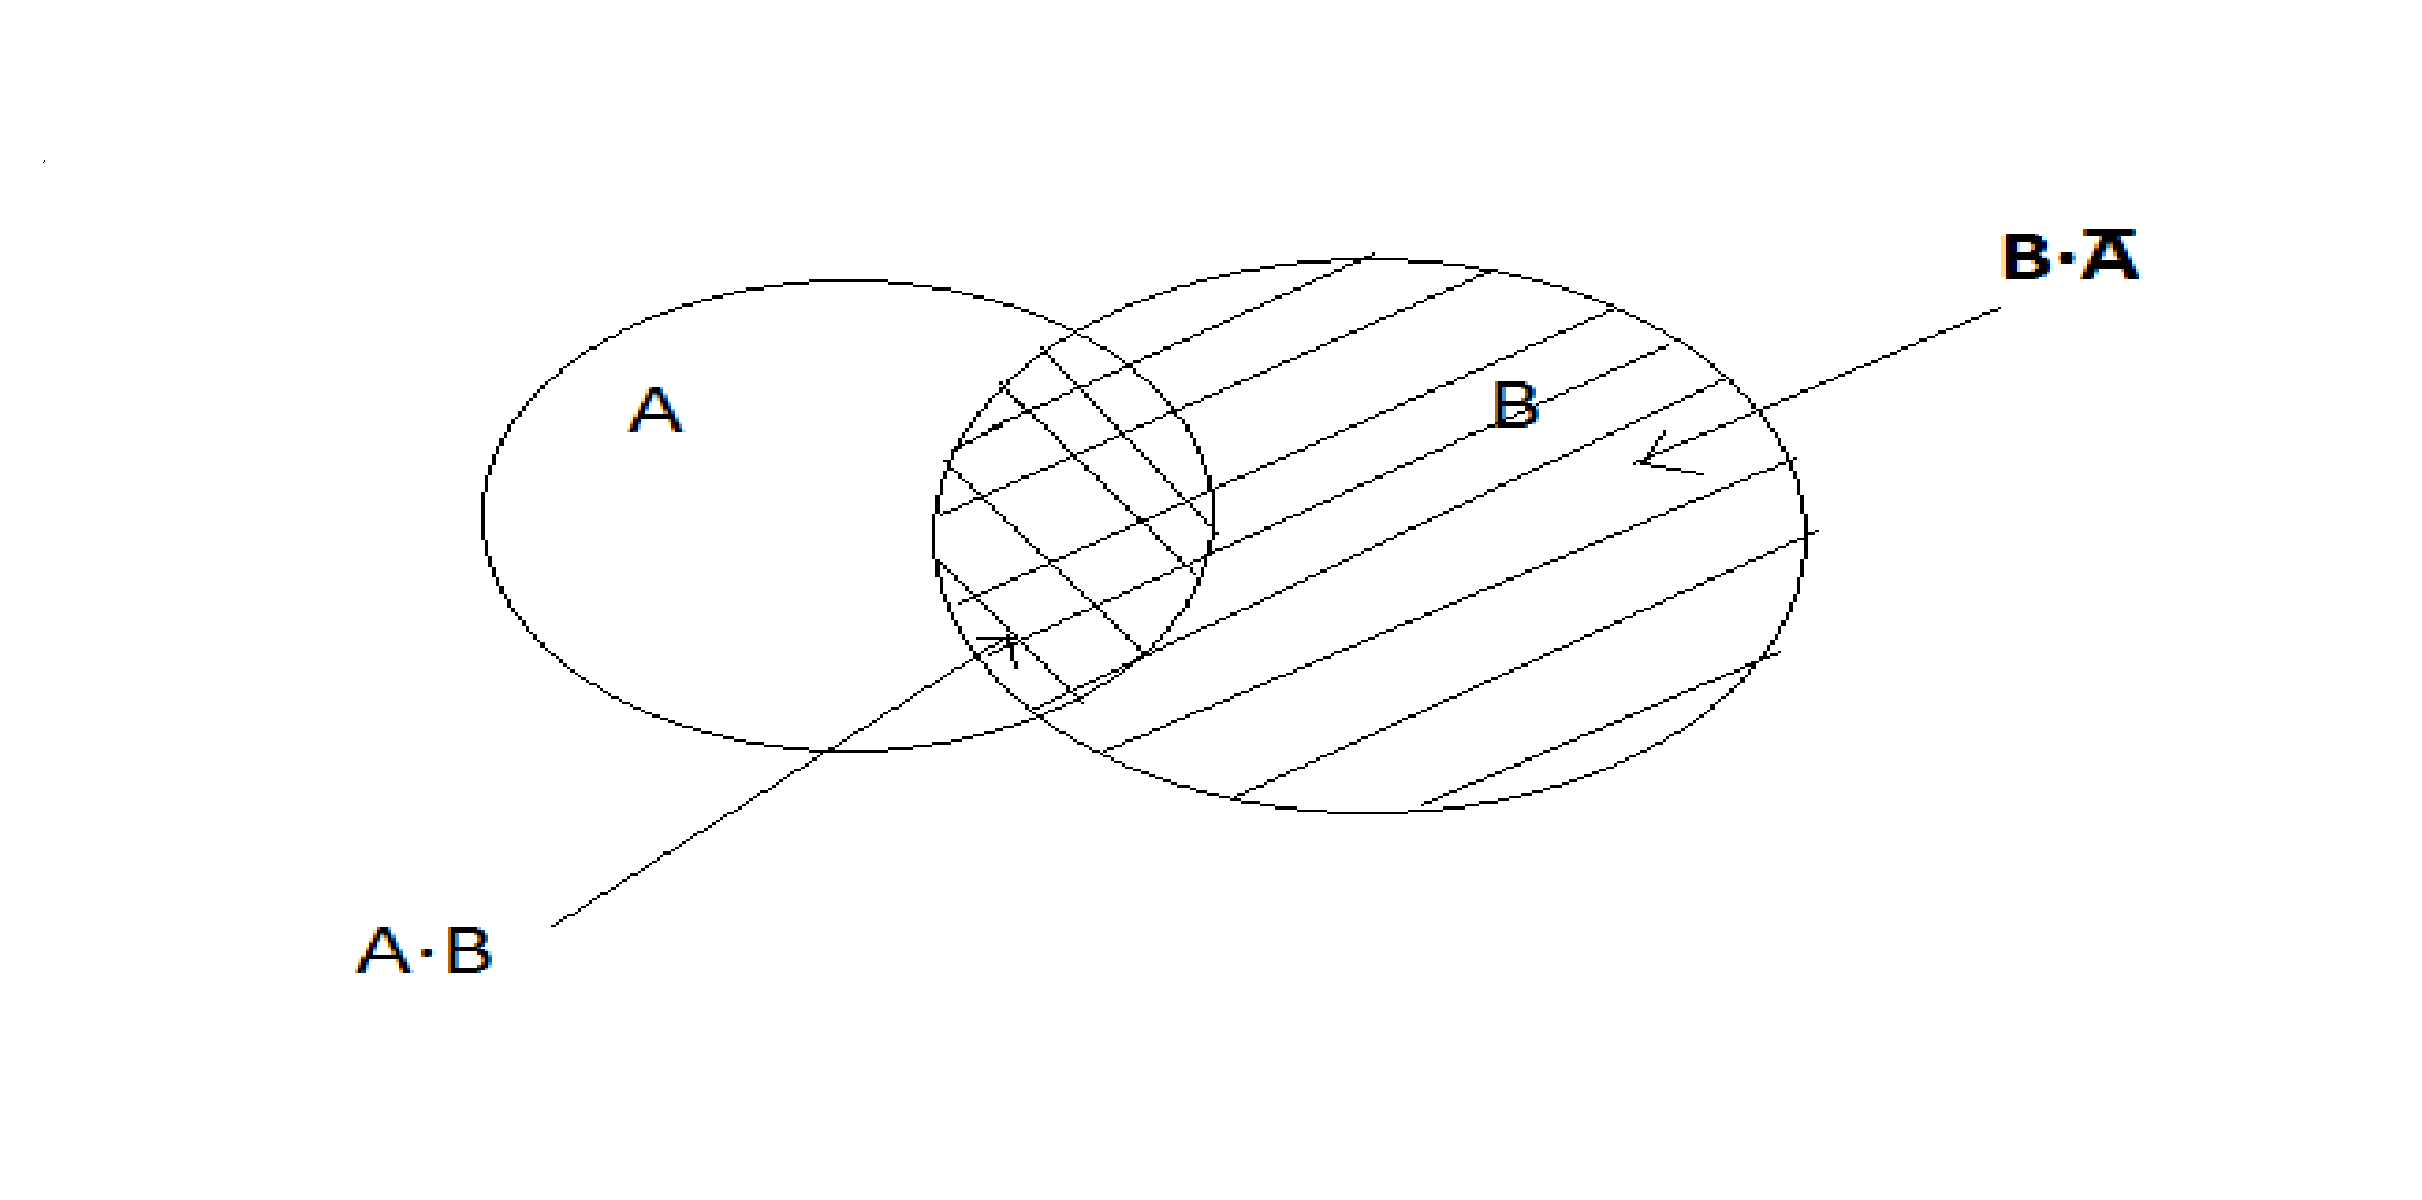
\includegraphics[scale=0.1]{x.png}\\
\textit{\textbf{Определение}} \\События $A$ и $B$ несовместны если $(A \cup B)$ =  $\emptyset$.\\
(То есть не могут произойти одновременно)\\
\textbf{Пример\\}Бросок кости $A$ -- не менее 3 очков, $В$ -- не более 4 очков,$\overline{A}$ -- менее 3 очков(1 или 2), $A$ + $B$ = {$\sigma$}, $A$ $\cdot$ $B$ = $3$ или $4$ очка.\\
\textbf{Пример}\\Выстрел по мишени. $A$ -- попадание, $B$ -- промах,  $A$ $\cdot$ $B$ = $\emptyset$.\\
$A$ + $B$ = $B$ + $A$\\
($A$ + $B$) + $C$ = $A$ + ($B$ + $C$)\\
$A$ $\cdot$ $B$ = $B$  $\cdot$ $A$\\
\textit{\textbf{Определение}}\\Пространство элементарных событий называется дискретным, если оно состоит из конечного числа точек, или из бесконечного числа точек, которые могут быть занумерованы последовательно(Счетное число точек).\\
\textbf{Пример}\\Предыдущий пример -- конечное число точек.\\
Теперь попробуем ввести вероятность, то есть число, которое характеризует степень обьективной возможности события.\\
\textit{\textbf{Определение}}\\Пусть дано дискретное пространство элементарных событий {$\sigma$} с точками $E_{1}$, $E_{2}$, $E_{3}$ . . .  Предполагаем, что с каждой точкой $E_{i}$ (событием) связано число, называемое вероятностью $E_{i}$ и обозначаемое P($E_{i}$), такое что:\\ 
1)$P$($E_{i}$) $\geq$ $0$  \\
2)$P$($E_{1}$) + $P$($E_{2}$) + . . . = $1$\\
Вероятность любого события $A$ есть сумма вероятностей элементарных событий из которых оно состоит.\\
1)$P(\sigma)$ = $1$\\
2)$P(\emptyset)$ = $0$\\
3)0 $\leq$ $P(A)$ $\leq$ $1$\\
%начало страницы 3
Как определить вероятность события в общей теории не постулируется. Об этом надо специально договариваться. Чаще всего встречается схема случаев.\\
Пусть  пространство эементарных событий состоит из n точек, причем все они равновозможны, то есть  по условиям симметрии есть основание считать, что ни одно из них не является обьективно более возможным, чем другие. Напомним, кроме того, что элементарные  события  
несовместны. Такие элементарные события обычно называют случаями.\\
\textbf{Пример}\\Орел и решка при броске монеты. Появляется для любой  из карт тщательно перетасованной колоды.\\
Пусть событие $А$ состоит из $m$ точек (эти $m$ случаев называются благоприятными событию $A$). Тогда вероятность $P(A)$  =$\frac{m}{n}$\\
\textbf{Пример}\\Бросок игральной кости. $A$  -- выпадение четного числа очков.\\$n$ =$6$, $m$ = $3$ ($2$, $4$, $6$) , следовательно, $P(A)$ = $\frac{3}{6}$ = $\frac{1}{2}$ \\
В других сиуациях, не сводящихся к схеме случаях, вероятность определяется по другому(например плотник, землемер, штурман измеряют расстояния -- одно и тоже, но делают это по разному). При этом все способы 
с корнями уходят в опыт.\\
Пусть производится n опытов, в каждом из которых может появится событие $А$. Частотой события $А$ называется отношение числа опытов, в которых появилось $А$ к общему числу опытов. Частоту часто называют статистической вероятностью.\\ 
 $0$ $\leq$ $P^*$($A$) $\leq$ 1, $P^*$($A$) = $\frac{m}{n}$\\
Так определенная статистическая вероятность носит случайный характер. Но при росте n она стабильно около некоторого значения. При n  $\rightarrow$  $\infty$ с практической достоверностью (то есть , вероятность ошибки сколь угодно мала) можно утверждать, что частота события будет сколько угодно мало отличаться от вероятности его в отдельном опыте. Более подробно это рассмотрим потом.\\
%начало страницы 4
\newpage
\begin{center}
$\textbf{Факты из комбинаторики}$
\end{center}
Число размещений с повторениями. $\overline{A^k_n}$ = $n^k$ , 
где $n$ -- количество типов элементов -- группы по $k$ элементов с учетом порядка(число трехзначных чисел в десятичной системе счисления равно $10^3$ - $10^2$).\\
Число размещений без повторений $A^k_n$ = $\frac{n!}{(n-k)!}$\\
$\textbf{Пример}$ \\$12$ человек учавствует в соревновании. Сколько вариантов распределения медалей. $\overline{A^3_{12}}$  = 12$\cdot$11$\cdot$10  = 1320\\
Число сочетаний без повторений  $C^k_n$ = $\frac{n!}{(n-k)!(k)!}$\\
$\textbf{Пример}$ \\$12$ команд. Сколько способов сформировать финальную группу из $3$ команд без учета мест?\\
  $C^3_{12}$  = $\frac{ 12\cdot11\cdot 10 }{2\cdot3} $ = $220$\\
Число  перестановок из $n$ различных элементов $P_n$ = n! = ${A^n_n}$\\
Число перестановок из $n$ = $n_1$ + $n_2$ +  $n_3$ . . .  + $n_k$ элементов, $n_1$ -- $1$ типа, $n_2$ -- $2$ типа, . . . $n_k$ -- $k$--го типа,\\
P($n_1$,  $n_2$, . . .  $n_k$) = $\frac{n!}{{n_1}!{n_2}!. . .{n_k}!}$\\
\textbf{Пример}\\ 8 ладей расстанавливаются на доске. Какова вероятность, что никакие две не бьют друг -- друга?\\
Сколько способов расположить ладей на шахматной доске что бы они не били друг друга? На каждой горизонтальной по одной. Пусть  на первой горихонтали она стоит на позиции $a_1$,  на второй на позиции $a_2$ и так далее.\\
($a_1$, $a_2$, ... $a_8$)  -- перестановка чисел $1,2\ .\ .\ .\ $8\\
То есть благоприятных случаев $P_8$ = $8$!\\
$P$ = $\frac{8!}{ 8^2 \cdot (8^2 - 1) \cdot (8^2 - 2)  \ .\ .\ . \   (8^2 - 7)} $  $\approx$   9 $\cdot$  $10^{-6}$\\
%начало страницы 5
Как определить вероятность если пространство элементарных собыий не является конечным? Чаcто здесь имеет смысл метод \underline{геометрической вероятности}. Если пространство  $\sigma$ может быть изображено геометрической фигуры и по условию опыта вероятность попадания точки (элементарного события) в любую часть области $\sigma$ пропорционально мере этой части (длинне, площади, обьему . . .) и не зависит от ее расположения и формы, то вероятность события А определяется как P(A) = $\frac{S_A}{S}$, где $S_A$ -- мера части области, попадание в которую благоприятствует событию $А$, $S$ -- мера всей области.\\
$\textbf{Пример}$\\Двое договорились встретится в определенном месте между 17 и 18 часами. Пришедший первым ждет второго 15 минут, после чего уходит. Определить вероятность встречи, если время прихода каждого независимо и равновероятно в течении этого часа.\\
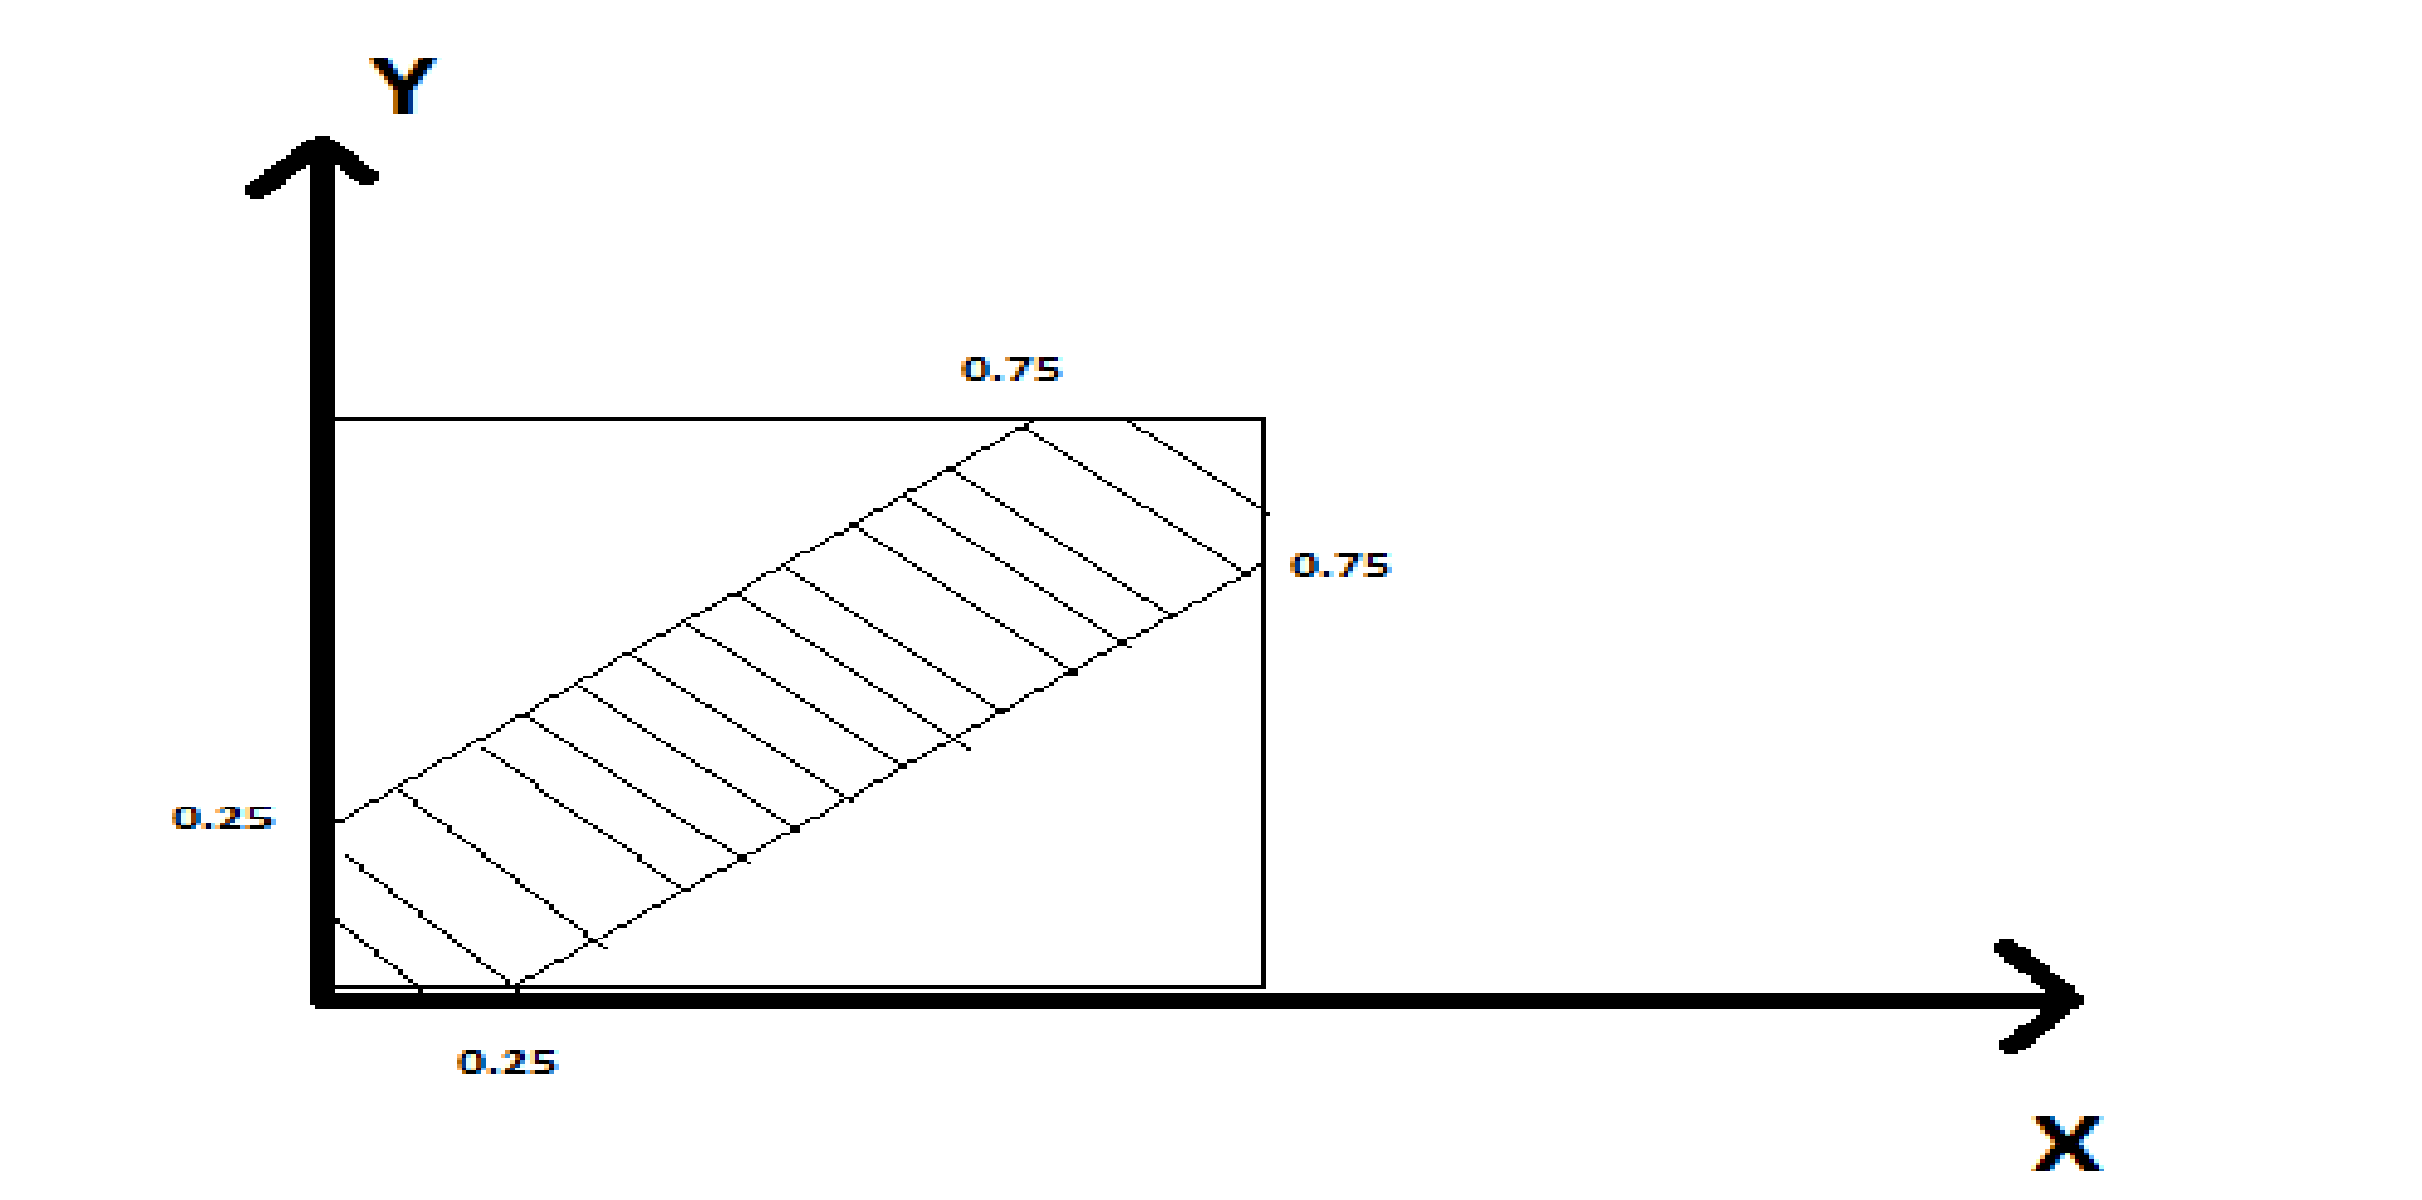
\includegraphics[scale=0.2]{page5.png}\\
Благоприятные исходы : $\abs{x - y} \leq \frac{1}{4}$\\
$\frac{1}{4} \leq x - y \leq \frac{1}{4}$\\	
$S_{области}$ = $1 - {(1 - \frac{1}{4})}^2$\\
$P$ = $\frac{1 - \frac{9}{16}}{1}$ = $\frac{7}{16}$
%начало страницы 6
\begin{center}
$\textbf{Парадокс де-Мере-Паскаля }$
\end{center}
Что вероятнее: при $3$ бросках игральной кости получить в сумме: $11$ или $12$ очков?\\
Рассуждение де-Мере: Cуммы $11$ и $12$ образуются при выпадении на костях следующих цифр: $12$ $=$ $6$ $+$  $5$ $+$ $1$ $=$ $6$ $+$ $3$ $+$ $3$ $=$ $5$ $+$ $4$ $+$ $3$ $=$ $5$ $+$ $5$ $+$ $2$ $=$ \\
$4$ $+$ $4$ $+$ $4$ (то есть $6$ вариантов);\\
$11\ =\  6\ +\ 4\ +\ 1\ =\ 6\ +\ 3\ +\ 2\ =\ 5\ +\ 5\ +\ 1\ =\ 5\ +\ 4\ +\ 2\ =\ 5\ +\ 3\ +\ 3\ =\ 4\ +\ 4\ +\ 2\ $(то есть $6$ вариантов);\\
То есть $11$ и $12$ должны быть равновероятны, но на опыте 11 появляется чаще.\\
На ошибку указал Паскаль: необходимо учитывать все возможные комбинации цифр, дающие в сумме 11 или 12.\\
Например $6\ +\ 5\ +\ 1\ =\ 6\ +\ 1\ +\ 5\ =\ 5\ +\ 1\ +\ 6\ =\ 5\ +\  6\ +\ 1\ =\ 1\ +\ 5\ +\ 6$\\
$=\ 1\ +\ 6\ +\ 5$ (то есть $6$ способов = $3$!). Аналогично, $6\ +\ 4\ +\ 2\  $($6\ =\ 3!$ способов), $6\ +\ 3\ +\  3\ $($3$ способа), $5$ $+$ $4$ $+$ $3$ ($6$ способов), $4$ $+$ $4$ $+$ $4$ ($1$ способ).\\
$P_{11}$ = $\frac{6 +  6 + 6 + 3 + 3 + 3}{6^3}$  $\textgreater P_{12}$.\\
\begin{center}
$\textbf{Сравнение статистик Больцмана, Бозе -- Энштейна, Ферми -- Дирака }$
\end{center}
Дано $k$ частиц и $l$ ячеек ($l$ $\textgreater$ $k$)\\
Найти вероятность того что:\\
	1)в определенных $k$ ячейках окажется по 1 частице\\
	2)в каких то ячейках окажется по одной частице\\
\textbf{Cтатистика Больцмана}
\begin{tabbing}
Ей подчиняется обычный газ.\\
Условия:\\
\qquad a)частицы различны\\
\qquad б)в любой ячейке может находится сколько угодно частиц\\
\end{tabbing}
1)Общее число исходов $l^k$(Так как любую частицу можно положить в любую ячейку). Благоприятных исходов $k!$, так как частицы различны и их можно переставлять.\\
Значит $P_1$ = $\frac{k!}{l^k}$\\
2)Теперь можно $k$ ячеек выбирать из $l$. (То есть число сочетаний k из общего числа l).То есть число благоприятных исходов равно $C^k_l \cdot k!$\\
$P_2$ = $\frac{C_l^k\cdot k!}{l^k}$\\

\textbf{Cтатистика Бозе-Энштейна}
\begin{tabbing}
Ей подчиняется обычный газ.\\
Условия:\\
\qquad a)частицы различны\\
\qquad б)в любой ячейке может находится сколько угодно частиц\\
\end{tabbing}
%начало страницы 7
Общее число исходов.\\
Перестaвив ячейки в ряд, границы определим перегородками, которых $l + 1$. Если поменять местами две частицы, то нового распределения не получится, так как частицы неразличимы. Если поменять местами две перегородки, то тоже ничего нового не получится, так как все перегородки одинаковы. Если же поменять местами перегородку и частицу, то получится новое распределение. Две крайние перегородки закреплены, поэтому в перестановке учавствует $ l - 1$ перегородок и к частиц, то есть  $k + 1 - l$ элементов.\\
Число перестановок равно : $\frac{(k + l - 1)!}{k!\cdot (l - 1)!}$\\
Число благоприятных исходов равно:\\
1)Так как перестановка частиц не дает нового распределения, то благоприятный исход один(при фиксированных ячейках).\\
То есть $P_1$ =$\frac{1}{\frac{(k + l - 1)!}{k!\cdot(l-1)!}}$ = $\frac{k!\cdot(l-1)!}{(k + l - 1)!}$\\
2)Число благоприятных исходов равно числу способов выбрать $k$ ячеек из $l$, где будут частицы: $C^k_l$ = $\frac{l!}{k!(l - k)!}$\\
$P_2$ = $\frac{l!(k + l - 1)!}{k!(l - k)!k!(l - 1)!}$ \\
\\
\textbf{Cтатистика Ферми--Дирака}
\begin{tabbing}
Ей подчинен, например, электронный газ.\\
\qquad a)частицы неразличимы\\
\qquad б)в ячейке может находится не более одной частицы (принцип Паули).
\end{tabbing}
Общее число исходов -- это число способов выбать из $l$ ячеек $k$, где будут частицы, то есть $C^k_l$ = $\frac{l!}{k!\cdot(l - k)!}$\\
Число благополучных исходов
\begin{tabbing}
\qquad 1)Так как $k$  ячеек определены, а частицы неразличимы, то благополучный исход один.\\$P_1$ = $\frac{1}{C^k_l}$ = $\frac{k!(l - k)!}{l!}$\\
\qquad 2)Число благополучных исходов равно числу способов выбрать $k$ заполненных ячеек из $l$ \\ равно $C^k_l$, следовательно $P_2 = \frac{C^k_l}{C^k_l}$ = 1
\end{tabbing}
%начало страницы 8
\subsection{Основные теоремы теории вероятностей}
$\textbf{Теорема сложения верояностей}$
\begin{tabbing}
\qquad\qquad$P(A + B) = P(A) + P(B)  -  P(AB)$
\end{tabbing}
\underline{Доказательство:}(для дискретного пространства элементарных событий). Что - бы получить $P(A + B)$ надо сложить вероятности точек входящих в $A$, и точек, входящих в $B$, на каждую по одному разу. Точки из $AB$ сосчитали дважды, поэтому их надо вычесть.\\
Если $A$ и $B$ несовместны то $P(A+B)=P(A)+P(B)$.
Если$A_1,\ A_2,\ .\ .\ .\ A_n$ - попарно несовместны, то $P(\sum\limits_{i=1}^{n}A_i)$ = $\sum\limits_{i=1}^{n}P(A_i)$\\
\textit{\textbf{Определение:}}\\ Говорят, что события $A_1, \ A_2,\ .\ .\ .\ A_n$ образуют полную группу, если $A_1+A_2+.\ .\ .\ A_n=\sigma$.\\
\textbf{Следствие\ 1}\\ Если события $A_1,A_2,\ .\ .\ .\ A_n$ образуют полную группу попарно несовместных событий, то  $\sum\limits_{i=1}^{n}P(A_i)$ $=$ $1$\\
%???
\textbf{Следствие\ 2} \\Сумма веротяностей противоположных событий равна $1$: $P(A)\ +\ P(\overline{A})\ =\ 1$\\
Если событий три:\\
$P(A+B+C)\  = \ P(A)\ +\ P(B)\ +\ P(C)\ -\ P(AB)\ -\  P(AC)\ -\ P(BC)\ +\ P(ABC)$\\
$P(\sum\limits_{i=1}^{n}A_i)$ = $\sum\limits_{i=1}^{n}P(A_i)$ - $\sum\limits{i,j}P(A_iA_j)$ $+$ . . . $+(-1)^{n-1}P(A_1,A_2, .\ .\ .\ A_n)$\\
$\textbf{Пример}$\\  Есть $100$ карточек с числами $1,\ 2,\ 3,\ .\ .\ .\ 100.$ Случайно выбирается одно из них.Событие $A$ -- число делится на $2$, $B$ -- делится на $3$. Найти вероятность $P(A+B)$.\\
\\
$P(A)\ =\ \frac{50}{100},\ P(B)\ =\ \frac{33}{100}$.\\  $AB$ -- делится на $6$: $P(AB)\ =\ \frac{16}{100}$. \\$P(A+B)\ =\ \frac{50}{100}\ + \frac{33}{100}\ -\frac{16}{100}=\frac{67}{100}$. \\\\
%начало страницы 9
\begin{center}
$\textbf{Торема умножения вероятностей }$
\end{center}
\textit{\textbf{Определение}}\\Событие $A$ называется независимым от события $B$, если вероятность события $A$ не зависит от того, произошло событие $B$ или нет, и зависимым, если вероятности $A$ меняются в зависимости от того, произошло событие $B$ или нет.\\
\textbf{Пример\ 1 }\\Бросание 2 монет. $A$ -- орел на первой монете, $B$ -- орел на второй монете. Эти события независимы.\\
\textbf{Пример\ 2 }\\Охотник, имеющий один патрон попадает в цель (cобытие $A$). Событие $B$ -- лев ловит добычу -- зависимые, если добыча -- охотник.\\
\textit{\textbf{Определение}}\\Вероятность события $A$, вычисленная при условии, что имело место событие $B$ -- называется условной вероятностью события $A$, и обозначается $P(A|B)$, или $P_B(A)$(считается $P(B)$ $\neq$ $A$). Условие независимости события $A$ от $B$ это $P(A|B)\ =\ P(B)$.\\
$\textbf{Теорема}$\\ $P(A\cdot B)\ =\ P(A)\cdot P(B|A)$.\\
\underline{Доказательство:}\\Для схемы случаев. Пусть в результате опыта возможно $n$ исходов, событие $A$ благоприятных $m$ исходов, событие $B$ -- $k$ исходов, и событие $A$, и событие $B$ -- $l$ исходов. $P(A\cdot B)\ =\ \frac{l}{n}$, $P(A)\ =\ \frac{m}{n}$. Если известно, что $A$ происходит, то из $n$ остальных возможных исходов, из них $l$ блокируют событие $B$, то есть  $P(A|B)=\frac{l}{m}$. То есть $P(A\cdot B) = P(A)\cdot P(B)$.\\
Ясно, что $P(A\cdot B) = P(B)\cdot P(A|B)$\\
\textbf{Следствие\ 1}\\Если событие $A$ не зависит от события $B$, то и событие $B$ не зависит от события $A$.
\begin{tabbing}
Известно, что $P(A)$ = $P(A|B)$. Считаем, что $P(A)$ $\neq$ $0$.\\
\end{tabbing}
\begin{equation*} 
 \begin{cases}
   $P(AB)$ = $P(A)P(B|A)$\\
   $P(AB)$ = $P(B)P(A|B)$
 \end{cases}
\end{equation*}
Следовательно, $P(A)P(B|A)$ = $P(B)P(A)$, следовательно\\
(при условии $P(A)$ $\neq$ $0$) $P(B|A)=P(B)$\\
То есть, свойство зависимости или независимости взаимно.\\
\textbf{Следствие\ 2}\\ Для независимых событий $P(A\cdot B)$ $=$ $P(A)\cdot P(B)$\\
Замечание: Эта формула может быть взята за определение независимых событий.\\
Умножение для $n$ событий.\\ $P(A_1, A_2, .\ .\ .\ .\ , A_n)$=$P(A_1)\cdot P(A_2|A_1) \cdot P(A_3|A_1A_2) \ .\ .\ . \ P(A_n|A_1,A_2 .\ .\ A_n)$\\
\textit{\textbf{Определение}}\\События $A_1, A_2, .\ .\ .\ , A_n$ называются независимыми в совокупности, если :\\ $P(A_1)\cdot P(A_2) \cdot .\ .\ .\  P(A_n)$\\
Замечание: это определение эквивалентно следующему: события независимы в совокупности, если любое из них не зависит любой совокупности остальных.\\
%начало страницы 10
$\underline{Замечание}$ Независимость в совокупности не эквивалентна попарной независимости событий\\
\textbf{Пример\ 1 }(Пример Берштейна): \\Имеется 4 шара. Красного, желтого, зеленого и трехцветный, имеющий красный, жёлтый и зелёный цвета на себе.Событие К -  вынули шар, на котором красный цвет, событие Ж - есть желтый, событие З - зелёный. $P($K$)=\frac{1}{2}$ = $P($Ж$)$ = $P($З$)$\\
Вероятность того, что вынули шар одновременно с двумя цветами = $P($K$\cdot$Ж$)\ =\frac{1}{4}$ = $P($К$)\cdot P($Ж$)$,  $P($K$\cdot$З$)\ =$  $P($К$)\cdot P($З$)\  = \  \frac{1}{4}$, $P($Ж$\cdot$З$)\ =$  $P($Ж$)\cdot P($З$)\  = \  \frac{1}{4}$.Вероятность того, что выпадет три цвета равна $P($К$\cdot$Ж$\cdot$З$)$ = $\frac{1}{4}\neq\\ \neq\ P($К$)\cdot P($Ж$) \cdot P($З$)=\frac{1}{8}$ То есть они попарно независимы, но зависимы в совокупности.\\
\textbf{Пример\ 2}\\
Техническое устройство отказывает с вероятностью $p=0.5$. Сколько раз его надо продублировать, что бы вероятность отказа установки была $q < 0.1$?\\
$P=p^n<0.1=q$, $n > \frac{ln(q)}{ln(p)}$\\
Суммы и произведение вероятностней часто работают вместе.\\
\textbf{Пример\ 3}\\ Пусть все элементы отказывают независимо от комбинаций других. Чему равна вероятность отказа цепи?\\
$P(A+B_1B_2+C_1C_2C_3)=P(A)+P(B_1)\cdot P(B_2)+P(C_1C_2C_3)-P(AB_1B_2)-P(AC_1C_2C_3)-P(B_1B_2C_1C_2C_3)+P(AB_1B_2C_1C_2C_3)$\\
\newpage
\begin{center}
$\textbf{Формула полной вероятности }$
\end{center}
\textit{\textbf{Определение}}\\Говорят, что события $H_1$, $H_2$, . . . $H_n$ образуют полную группу, если $H_1+H_2+$. . .$H_n$ -- достоверное событие.\\
Пусть $H_1$, $H_2$, . . . $H_n$ -- полная группа попарно несовместимых событий. Эти события будем называть гипотезами. Пусть надо найти вероятность события $A$, которое может произойти вместе с одной из гипотез. Тогда $P(A)=\sum\limits_{i=1}^{n}P(H_i)\cdot P(A|H_i)$\\
Так как $H_1$, . . .$H_n$ -- полная группа. $A$ $=$ $H_1A\ +H_2A\ +$  . . .  $+H_nA$. $H_1,$. . .$H_n$ -- попарно несовместные, следовательно $H_1A,$ . . . $H_nA$ -- несовместны, следовательно $P(A)=P(H_1A) +$. . . $P(H_nA)$ $=$ $\sum\limits_{i = 1}^{n} P(H_iA)$, следовательно, по теореме умножения $P(A)=\sum\limits_{i = 1}^{n}P(H_i)\cdot P(A|H_i)$\\
\textbf{Пример\ }\\По самолету производится 3 выстрела. Вероятность попадания при первом $0.4$, при втором - $0.5$, при третьем -- $0.7$. Для вывода самолета из
%начало страницы 11
 строя завведомо достаточно 3 попаданий. При первом попадании самолет выходит из строя с вероятностью $0.2$, при двух -- $0.6$. Найти вероятность того, что в результате трех выстрелов самолет будет выведен из строя.\\
$H_i$ -- в самолет попал $i$--й снаряд, $P(H_0)=0.6\cdot0.5\cdot0.3=0.09$. $P(H_1)=0.4\cdot0.5\cdot0.3+0.6\cdot0.5\cdot0.3+0.6\cdot0.5\cdot0.7=0.36$\\
$P(H_2)=0.6\cdot0.5\cdot 0.7+0.4\cdot0.5\cdot0.7+0.4\cdot0.5\cdot0.5=0.41$, $P(H_3)=0.4\cdot0.5\cdot0.7=0.14$\\
$P(A)=0.36\cdot0.2+0.41\cdot0.6+0.14\cdot1=0.458$\\
\begin{center}
$\textbf{Формула Байеса }$
\end{center}
Пусть событие $A$ может произойти с одним из $n$ попарно несовместимых событий $H_1, H_2, .\ .\ .\ H_n$, образующих полную группу. Вероятности гипотез до опыта известны -- $P(H_1)$, . . . $P(H_n)$ (априорные вероятности). Произведен опыт, в результате которого произошло событие $A$. Как следует изменить вероятности гипотез в связи с появлением $A$ (то есть найти постериорные вероятности $P(H_i|A)$?
$P(AH_i)=P(A)\cdot P(H_i|A) = P(H_i) \cdot P(A|H_i)$, следовательно $P(H_i|A) = \frac{P(H_i) \cdot P(A|H_i)}{P(A)}$.\\
Итого: $P(H_i|A) = \frac{P(H_i)\cdot P(A|H_i)}{ \sum\limits_{j=1}^{n}P(H_j)\cdot P(A|H_j) }$\\
\\
\textbf{Пример\ }\\
В первой урне 5 белых и 10 черных шаров.Во второй - 3 белых и 7 черных. Из второй в первую переложили $1$ шар, а затем из второй вынули один шар. Оказалось что он белый. Найти вероятность того, что был переложен белый шар\\
$H_1$ -- переложили белый, $H_2$ -- черный, $P(H_1)=\frac{3}{10}$, $P(H_2)=\frac{7}{10}$. $P(A|H_1)=\frac{6}{11}$, $P(A|H_2)=\frac{5}{11}$\\
 $P(A)=\frac{3}{10}\cdot \frac{6}{11} + \frac{7}{10} \cdot \frac{5}{11}$, $P(H_1|A)$ = $\frac {\frac{3}{10}\cdot \frac{6}{11} }   {\frac{3\cdot 6}{10\cdot11} + \frac{7\cdot5}{10\cdot11}  }$ = $\frac{18}{18 + 35}$\\
\textbf{Пример\ }\\
Известно, что $5\%$ мужчин и $0.25\%$ женщин -- дальтоники. Наугад выбранное лицо страдает дальтонизмом. Какова вероятность того, что это мужчина?\\
$P(H_1) = P(H_2) = \frac{1}{2}$\\
$P(A|H_1) = 0.05$, $P(A|H_2) = 0.0025$, $P(H_1|A) = \frac{\frac{1}{2} \cdot 0.05}{ \frac{1}{2} \cdot 0.05 + \frac{1}{2} \cdot 0.0025 } = \frac{20}{21}$\\
%начало страницы 12
\subsection{Повторение опытов}
В самом начале развития теории вероятностей выяснилась фундаментальная роль одной математической схемы, изученной швейцарцем Яковом Бернулли.\\
Схема такая: проведем последовательность испытаний, в каждом из которых вероятность события $A$ одна и та -- же($p$). Испытания независимы, то есть вероятность выявления события $A$ в каждом из них не зависит от того, появилось оно или нет в других испытаниях.\\
\textbf{Пример\ }\\ $2$ игрока играют в шахматы $3$ партии. Вероятность выигрыша первого $p = \frac{2}{3}$. Найти вероятность того, что он выиграет $2$ партии.\\
Это можно осуществить : $P(A_1A_2\overline{A_3} + A_1\overline{A_2}A_3 + \overline{A_1}A_2A_3)=\frac{2}{3}\cdot\frac{2}{3}\cdot\frac{1}{3} + \frac{2}{3}\cdot\frac{1}{3}\cdot\frac{2}{3} + \frac{1}{3}\cdot\frac{2}{3}\cdot\frac{2}{3} = \frac{4}{9}.$\\
В общем виде: вероятность того, что в $n$ опытах событие произойдет $m$ раз $P_n(m)$ равна $A_1A_2.\ . \ . \ A_m\overline{A_{m+1}}.\ .\ .\ \overline{A_n} + 
A_1A_2.\ . \ . \ \overline{A_m} A_{m+1} \overline{A_{m+2}} .\ .\ .\ \overline{A_n} +
\ \ \ .\ .\ .\ 
+\overline{A_1}\overline{A_2}.\ . \ . \ \overline{A_{n-m}} {A_{n-m+1}} .\ .\ .\ A_n$
В каждую комбинацию $A$ входит $m$ раз %****
Число комбинаций $C^m_n$, все комбинации несовместны, следовательно $P_n(m) = p^mq^{n-m} + p^mq^{n-m} + .\ .\ . = C^m_np^mq^{n-m}$ , где $q = 1 - p$.\\
Так как по форме $P_n(m)$ %не понял
член разложения бинома $(q+p)^n$ распределение веротяностей такого вида называется биноминальным распределением.\\
\textbf{Пример\ }\\
Два шахматных игрока, 10 результативных партий (ничьи не учитываются), Вероятность выигрыша первого -- $\frac{2}{3}$, второго -- $\frac{1}{3}$. Найти вероятность выигрыша
 всей игры первым?\\
$P_{выигрыша\ 1} = P_{10}(6) + P_{10}(7) + P_{10}(8) + P_{10}(9) +  P_{10}(10)$ = $\frac{2^6}{3^{10}}\cdot(210+240+180+80+16) = \frac{2^6\cdot241}{3^{9}}$
$P_{выигрыша\ 2} = P_{10}(6) + P_{10}(0) + P_{10}(1) + P_{10}(2) +  P_{10}(3)  +  P_{10}(4)$ = $\frac{1507}{3^{9}}\cdot(210+240+180+80+16)$\\
То есть вероятность выигрыша первой партии у первого в два раза больше чем у второго, вероятность выигрыша матча у первого в 10 раз больше, чем у второго.\\
\textbf{Замечание\ } \\
$\sum\limits_{m = 0}^{n}P_n(m) = 1$, $(p+q)^n=1$, $p+q = 1$, следовательно, $(p+q)^n = \sum\limits_{m = 0}^{n}P_n(m)  = \sum\limits_{m = 0}^{n}C^m_np^mq^{(n-m)}$ -- Бином Ньютона.\\
%начало страницы 13
\section{Случайные величины}
\textit{\textbf{Определение}}\\
Функция, определённая на пространстве элементарных событий называется случайной величиной.\\
\textit{\textbf{Определение}}\\
Случайная величина называется дискретной, если она определена на дикретном пространстве элементарных событий.\\
Замечание: лучше бы было называть случайные величины функциями случая\\
\textbf{Пример\ }\\Дискретная случайная величина. Число тузов у одного игрока при игре в бридж, число совпадающих дней рождения в группе из $n$ человек.\\
Обозначать случайные величины будем буквами $X, Y$, . . . и их значения $x, y$ . . . .
Пусть $X$ -- случайная величина. $x_1, x_2,$ . . .  --  ее значения. Совокупность всех элементарных событий, на которых $X$ принимает значение $x_i$ образует событие $X=x_i$.
Его вероятность обозначается $P(X=x_j) = p_j$. Соотношение, устанавливающее связь между значениями случайных величин и их вероятностями называется законом распределения случайной величины. Самой простой формой закона распределения для случайной величины является ряд распределения то есть таблица распределения, в которой сведены значения случайной величины и их вероятности. Для наглядности это часто изображают на графике и точки соединяют отрезками прямых. Получившаяся фигура называется многоугольником распределения. Так как события $X=x_j$ -- несовместимы и образуют полную группу, то $\sum\limits_{i = 1}^{n}p_i = 1$.\\
\textbf{Пример\ }\\
Баскетболист бросает мяч в кольцо до первого попадания, либо пока не сделано 3 броска. Вероятность попадания при одном броске равна $0.7$.\\
%началоо страницы 14
\begin{center}
$\textbf{Функция распределения }$\\
\end{center}
Вероятность $P(X=x)$ часто использовать неудобно. Используют вероятность $P(X<x).$\\
\textit{\textbf{Определение}}\\
Функция распределения (интегральная функция распределения) или интегральный закон распределения или рапределение накопленой веротяности) - это функция на вещественной оси, определяемая следующим образом: $F(x)=P(X<x)$\\
$F(x)$ полностью характеризует случайную величину с вероятностной точки зрения, то есть это форма закона распределения.\\
Свойства:\\
1)$F(x)$ - неубывающая функция (то есть при $x_1 < x_2$ $F(x_1) \leq F(x_2)$\\
2)$\displaystyle{  \lim_{x\to{-\infty}}  } F(x) = 0$\\
3)$\displaystyle{  \lim_{x\to{+\infty}}  } F(x)  = 1$\\
4)$F(x)$ непрерывна слева. $\displaystyle{ F(x_i) = \lim_{x\to{x_i - 0}} F(x) }$ \\
\textit{\textbf{Определение}}\\
Случайная величина называется непрерывной, если ее функция распределения непрерывна.\\
Для дискретной случайной величины :$F(x) = \sum\limits_{x_j < x}P(X=x_j)$\\
\textbf{Пример\ }\\
Случайная величина -- площадь разрушений, наносимых бомбой. Значение этой случайной величины непрерывно заполняет промежуток от $0$ $\pi R^2$ ($R$ -- радиус действия). Но в точках $0$ и $\pi R^2$ у функции распределения скачки, так как этим значениям соотвествуют конечные вероятности (вероятности положений 1 и 3 соответственно) круга разрыва.\\
%начало страницы 15
\begin{center}
$\textbf{Вероятность попадания точки на отрезок. }$
\end{center}
$P(\alpha \leq  x <  \beta) = P(x < \beta) - P(x < \alpha) = F(\beta) - F(\alpha)$\\
\textbf{Замечание\ } \\
$P(\alpha \leq  x \leq  \beta) = F(\beta) - F(\alpha) + P(x = \beta)$\\
$P(x = \alpha)=$   $\displaystyle{  \lim_{\beta \to{\alpha}}} $           $ P(\alpha \leq x < \beta) =$    $\displaystyle { \lim_{\beta \to {\alpha}}} (F(\beta) - F(\alpha))$\\
Если слева величина непрерывна, то $P(x=\alpha)=0$.\\
\begin{center}
$\textbf{Плотность распределения }$\\
\end{center}
Пусть непрерывная случайная величина имеет дифференцируемую функцию распределения. Тогда $P(x<X<x + \Delta x) =  F(x + \Delta x) - F(x)$\\
\textit{\textbf{Определение}}\\ $f(x) =$ $\displaystyle { \lim_{{\Delta x} \to {0}}}$ $\frac{P(x<X<x+\Delta x)}{\Delta x}$ = $F'(x)$ -- плотность вероятности (плотность распределения).\\
$F(x)$ -- первообразная для $f(x)$. Так как $F(-\inf)=0$, то константа в первообразной выбирается однозначно.\\
$F(x) = \int\limits_{-\infty}^{x}f(x)dx$\\
Найдем $P(\alpha < X < \beta)$ через $f(x)$. Так как вероятность одного значения непрерывной случайной величины равна нулю: $P(\alpha <  X < \beta) = P(\alpha \leq  X < \beta) = F(\beta) - F(\alpha)=  \int\limits_{-\infty}^{\beta}f(x)dx -   \int\limits_{-\infty}^{\alpha}f(x)dx =  \int\limits_{\alpha}^{\beta}f(x)dx$.
Геометрически $P(\alpha<x<\beta)$ -- это площадь.\\
%начало страницы 16
Свойства плотности вероятности:\\
1)$f(x)\geqslant 0$ (следует из того, что $F(x)$ неубывает\\
2)$  \int\limits_{-\infty}^{\infty}f(x)dx=1$(так как $F(\infty)$)\\
То есть график плотности вероятности выше оси абсцисс, а полная площадь равна 1.\\
\textbf{Пример\ }\\
\begin{equation*} 
f(x)=
 \begin{cases}
   a \cdot cos(x), -\frac{\pi}{2} \leq x \leq \frac{\pi}{2} \\
   0 , x < -\frac{\pi}{2} $ или $ x > \frac{\pi}{2}
 \end{cases}
\end{equation*}
$  \int\limits_{-\frac{\pi}{2}}^{\frac{\pi}{2}}a\cdot cos x dx = 2a = 1$, следовательно, $a = \frac{1}{2}$\\
\begin{equation*} 
F(x)=
 \begin{cases}
   0 , x < -\frac{\pi}{2}\\
   \frac{1}{2} \cdot (sin(x) + 1) , \frac{\pi}{2} \leq x \leq \frac{\pi}{2} \\
   1 ,  x > \frac{\pi}{2}
 \end{cases}
\end{equation*}
%начало страницы 17
\begin{center}
$\textbf{Числовые характеристики случайных величин. }$\\
\end{center}
Функция распределения или плотность полностью описывает случайную величину с вероятностной точки зрения.\\
\begin{tabular}[b]{ | l | l | l | }
\hline
Характеристика &  Дискретная & Непрерывная   \\
 &  сл. вел-на X  & сл.  вел-на X  \\
\hline
Мат ожидание &  $ \sum\limits_{k} x_kp_k$ & $\int\limits_{-\infty}^{\infty}xf(x)dx$\\
Дисперсия & $\sum\limits_{k}^{}(x_k-M(x))^2p_k$ & $\int\limits_{-\infty}^{\infty}(x- M(x))^2f(x)dx$\\
Начальный момент & $\sum\limits_{k} x^s_kp_k$ & $\int\limits_{-\infty}^{\infty}x^sf(x)dx$\\
порядка S& &\\
Центральный момент& $\sum\limits_{k}^{}(x_k-M(x))^sp_k$& $\int\limits_{-\infty}^{\infty}(x- M(x))^sf(x)dx$\\
порядка S& &\\
Мода&наиболее вероятное&значение, \\
& значение& в котором f(x)\\
& &максимально\\
Медиана&не определено&такое $X$= $Me$, что \\
& & $P(X < Me)=$\\
& & $=P(X > Me)$\\
Среднеквадратичное  & $\sigma(x) = \sqrt{D(x)}$ & $\sigma(x) = \sqrt{D(x)}$\\
отклонение $\sigma(x)$ & &\\
Коэффициент симметрии $S_k$ & $S_k$ = $\frac{\mu_3}{\sigma^3}$ &  $S_k$ = $\frac{\mu_3}{\sigma^3}$ \\
Эксцесс $E_x$ & $E_x$ = $\frac{\mu_4}{\sigma^4}$ & $E_x$ = $\frac{\mu_4}{\sigma^4} - 3$\\
\hline
\end{tabular}\\
\textit{\textbf{Определение}}\\
Математическое ожидание дискретной случайной величины (среднее значение) -- это число $M(X)(E(X), \overline{X} , <X>)$, определяется по формуле $M(X)=\sum\limits_{k}x_kp_k$, при условии, что ряд абсолютно сходится. Если ряд абсолютно расходится, то говорят что $X$ не имеет конечного математического ожидания. Пусть случайная величина может принимать одно из $N$ равновероятных \\ значений $x_1,x_2,$ . . .$x_n$. Тогда $p_i = \frac{1}{N}$ и $M(X) = \frac{\sum\limits_{i = 1}^{N}  x_i } { N }$ -- среднее арифметическое. Если значение не является равновероятным, то надо брать взвешенное среднее, что и сделано в определении. Аналогично с точечными массами и центром масс.\\
\textbf{Замечание\ } \\
$M(X)$ может быть значением случайной величины.\\
\textbf{Пример\ }\\
Испытываются однотипные приборы. Веротятность каждого пройти испытание равно p и независимы. Испытания заканчиваются после выхода из строя первого же прибора. $X$ -- число произведенных испытаний. Чему равно $M(X)$?\\
$P(X=k) = q\cdot p ^{k - 1}$, $q = 1 - p$.\\
$M(X) = 1\cdot q + 2q\cdot p + 3 q \cdot p^2 + .\ .\ .\ +k\cdot q\cdot p^{k-1}$ = $q(1+2p+3p^2 + \ .\ .\ )'$ = $q\cdot(\frac{p}{1-p}) ' = \frac{q}{{(1-p)}^2} = \frac{1}{q}$\\
%начало страницы 18
\textbf{Пример\ }\\
 Пример отсутствия конечного математического ожидания -- "Петербургская игра". Бросается монета до тех пор, пока не выпадет орёл. Если это случается при бросании c номером $r$, то игрок получит $2^r$ рублей. $x_r=2^r$, $p_r=2^{-r}$. $\sum\limits_{r = 1}^{\infty}  x_rp_r = \sum\limits_{r = 1}^{\infty} 1 = \infty$\\
\textit{\textbf{Определение}}\\
Мода -- координата максимума $f(x)$. Если кривая распределения имеет более одного максимума, то распределение называется полимодальным.\\
\textit{\textbf{Определение}}\\
Медиана : $P(X<Me) = P(X>Me)$, для непрерывной случайной величины.\\
\textit{\textbf{Определение}}\\
Квантиль порядка $p$ -- это значение $x_p$, соответствующее значению функции распределения равному $p$ $(F(xp)=p)$.Медиана - квантиль порядка $\frac{1}{2}$.\\
\textit{\textbf{Определение}}\\
Центрированной случайной величиной $X$, соответствующей величине $X$ называется отклонение случайной величины $X$ ее математического ожидания.($A$)
Как оценить разброс $X$ относительно среднего? Можно рассмотреть $M(A)$, но он оказывается равен 0.
$M(X - m_x) = \sum\limits_{i=1}^{n}(x_i-m_x)p_i=\sum\limits_{i=1}^{n}x_ip_i - m_x\sum\limits_{i=1}^{n}p_i = m_x - m_x = 0$\\
Поэтому используют $M((X-m_x)^2)$ = $D(X)$ = $Var(X)$\\
$D(X)= \sum\limits_{i=1}^{n} (x_i - m_x)^2p_i$ = $\sum\limits_{i=1}^{n}x_i^2 - 2m_x\sum\limits_{i=1}^{n}x_ip_i + m_x^2\sum\limits_{i=1}^{n}p_i = \sum\limits_{i=1}^{n}x_i^2p_i - m_x^2$\\
Для непрерывных величин: $D(X) = \int\limits_{-\infty}^{\infty}x^2f(x)dx - m_x^2$\\
Разброс характеризуется средним квадратичным отклонением: $\sigma(x) = \sqrt{D(x)}$\\
\textbf{Пример\ }\\
\begin{equation*} 
f(x)=
 \begin{cases}
   2x,  x \in [0, 1]\\
   0 , x \notin [0, 1]\\
 \end{cases}
\end{equation*}\\
$M(X) = \int\limits_{0}^{1}x\cdot 2x d x  = \frac{2}{3}$\\
$D(x) = \int\limits_{0}^{1}x^2\cdot 2x d x - \frac{4}{9} = \frac{1}{2} - \frac{4}{9} = \frac{1}{18}$\\
$\sigma(x) = \frac{1}{3\sqrt{2}}$
Чему равно $x_p$?\\
$F(x) = \int\limits_{0}^{\inf}2tdt = x^2$, $x^2 = p$, следовательно, $x_p = \sqrt{p}; M_e = x_\frac{1}{2} = \frac{1}{\sqrt{2}}$\\
%страница 19
Начальный момент порядка S: $\alpha_S$ = $\sum\limits_{k} x^s_kp_k$  = $\int\limits_{-\infty}^{\infty}x^sf(x)dx$\\
Центральный момент порядка S:  $\sum\limits_{k}^{}(x_k-M(x))^sp_k$  = $\int\limits_{-\infty}^{\infty}(x- M(x))^sf(x)dx$\\
Центральный и начальный моменты связаны: $\mu_2 = \alpha_2 - m_x^2$\\
$\mu_3 = \sum\limits_{i}^{n}(x_i-m_x)^3p_i =\sum\limits_{i}^{}x_i^3p_i - 3m_x\sum\limits_{i}^{ }x_i^2p_i + 3m_x^2\sum\limits_{i}^{ }x_ip_i - m_x^3\sum\limits_{i}^{ }p_i = \alpha_3 - 3 m_x \alpha_2 + 2m_x^3$\\
Можно определить моменты не относительно $m_x$, а относительно точки $a$: $M((x-a)^s)$.\\
Однако центрированные имеют преимущество в части : $D(X) = min M((x-a)^2)$\\
$M(X-a)^2$ = $\int\limits_{-\infty}^{\infty}(x-m_x+m_x-a)^2f(x)dx$ = $\int\limits_{-\infty}^{\infty}(x-m_x)^2f(x)dx + 2(m_x-a)\int\limits_{-\infty}^{\infty}(x-m_x)f(x)dx + (m_x - a)^2 \int\limits_{-\infty}^{\infty} f(x)dx = D(X) + (m_x-a)^2$, следовательно минимум достигается при $m_x=a$\\
Нечетные центральные моменты характеризуют симметрию распределения(кроме первого, который всегда ноль). Поэтому для характеристики симетрии выбирают третий центральный  момент.\\
Коэфициент симметрии: $S_k(x) = \frac{\mu_3}{\sigma^3}$.\\
Если симметрия относительно $m_x$, то $S_k = 0$.\\
Четвертый момент служит для характеристики крутости, то есть островерщинности или плосковершинности распределения.За стандартное распределение,  с которым проводится сравнение принято нормальное распределение: $f(x) = \frac{1}{\sqrt{2\pi}\sigma}\cdot e^{-\frac{(x-m_x)^2}{2\sigma^2}}$. Его эксцесс = $E_x = \frac{\mu_4}{\sigma_4} - 3$. Для нормального $E_x = 0$.\\
\textbf{Пример\ }\\
\begin{equation*} 
f(x)=
 \begin{cases}
   2x,  x \in [0, 1]\\
   0 , x \notin [0, 1]\\
 \end{cases}
\end{equation*}\\
$\alpha_3 = 2\int\limits_{0}^{1}x^4dx=\frac{2}{5}$, $\mu_3 = \alpha_3 - 3m_x\alpha_2 + 2m_x^3 = \frac{2}{5} - 3\cdot\frac{2}{3}\cdot\frac{1}{2} + 2 \cdot (\frac{2}{3})^3 = \frac{1}{135}$\\
$S_k = \frac{\mu_3}{\sigma_3} = -\frac{2}{5}\sqrt2$\\
$\mu_4 = 2\int\limits_0^1x^4dx=2\int\limits_0 ^1(x-\frac{2}{3})^5dx + \frac{4}{3}\int\limits_{0}^{1}(x-\frac{2}{3})^4dx$ = $\frac{1}{3^7} - \frac{2^6}{3^7} + \frac{4}{15} \cdot \frac{4^0}{3^5} + \frac{2^7}{5\cdot3^6}$ = $\frac{2^2}{3^3} - \frac{2^8}{3^3} + \frac{16}{5\cdot3^2} + \frac{2^9}{5\cdot3^2}$ $>0$.\\
Помимо важных отдельных моментов существенных значений имеет полный набор моментов ($\mu_n$ или $\alpha_n$). Часто проще найти полный набор %хз
, чем само распределение. А при весьма общих условиях набор моментов полностью определяет распределение вероятности.\\
$\textbf{Теорема}$\\
Если две плотности веротяности $f_1(x)$ и $f_2(x)$ -- непрерывные случайные величины имеют одинаковые моменты $\alpha$ и функция $f_1(x) - f_2(x)$ представляется сходящимся на $(-\infty;\infty)$ рядом по степеням $x$, то $f_1(x) = f_2(x)$.\\
\underline{Доказательство:}\\
Пусть $f_1(x) - f_2(x)= c_0 + c_1x + c_2x^2 +$ . . . =\\
$\int\limits_{-\infty}^{\infty} (f_1(x) - f_2(x))^2dx = \int\limits_{-\infty}^{\infty} (f_1(x) - f_2(x))(c_0 + c_1x + c_2x^2 + .\ .\ .\ .)dx$\\
$=c_0\int\limits_{-\infty}^{\infty}(f_1(x)-f_2(x))dx + c_1\int\limits_{-\infty}^{\infty}(xf_1(x) - xf_2(x)) + c_2\int\limits_{-\infty}^{\infty}(x^2f_1(x) - x^2f_2(x))  + $. . .  = \\
$c_0(1 - 1) + c_1(\alpha_1-\alpha_1) + c_2(\alpha_2 - \alpha_2) + $ . . . $=0$, следовательно, $f_1(x) = f_2(x)$.\\
\textbf{Замечание\ } \\ 
Для "смешанной"\  случайной величины формулы дискретной и непрерывной обьединяются для значений $0\leq x< 1$ -- плотность $f(x) = \frac{1}{2}$.\\
$M(X) = 0\cdot \frac{3}{8} + 1\cdot \frac{1}{8} + \int\limits_{0}^{1}x\cdot \frac{1}{2} dx = \frac{3}{8}$
%страница 21

\section{Различные законы распределения величин}
\subsection{Равномерные распределения}
Равномерно распределенная непрерывная случайная величина -- случайная величинп, у которой плотность вероятности постоянна на некотором интервале, а вне него равна нулю.\\
\textbf{Пример\ }\\
Колесо рулетки. Зафиксируем некоторое направление. Тогда угол под которым она останавливается -- случайная величина, равномерно распределенная в интервале $(0, 2\pi)$.\\
\textbf{Пример\ }\\
Производится взвешивание на весах с ценой деления 1 грамм. Если оказывается что вес заключен от $k$ до $k + 1$ грамм, тогда его можно принять за $(k + \frac{1}{2})$ и считать, что при этом допущенна ошибка $X$ -- случайная величина, равномерно распределенная на интервале $(-\frac{1}{2}, \frac{1}{2})$ грамм.\\

Пусть распределение $X$ равномерно на $(a, b)$.\\
\begin{equation*} 
f(x)=
 \begin{cases}
   c,   x \in [a, b]\\
   0 , x \notin [a, b]\\
 \end{cases}
\end{equation*}\\
$\int\limits_{a}^{b} c dx = c(b - a)$ = 1, значит $c = \frac{1}{b - a}$\\
Итого, \\
\begin{equation*} 
f(x)=
 \begin{cases}
   \frac{1}{b - a},   x \in [a, b]\\
   0 , x \notin [a, b]\\
 \end{cases}
\end{equation*}\\
Значит, \\
\begin{equation*} 
f(x)=
 \begin{cases}
   c,   x \in [a, b]\\
   0 , x \notin [a, b]\\
 \end{cases}
\end{equation*}\\
Итого, \begin{equation*} 
F(x)=
 \begin{cases}
    0,   x \leq a\\
   \frac{x - a}{x - b} , a < x < b\\
   1, x \geq b\\
\end{cases}
\end{equation*}\\
$M(X) = \int\limits_{a}^{b}\frac{x}{b-a}dx = \frac{a + b}{2}$
В силу симметричности $M_e= \frac{a+b}{2} = M(x)$\\
Моды это распределение не имеет.\\
$D(X) = \frac{1}{b - 1} \int\limits_{x}^b(x - \frac{a + b}{2})^2dx = \frac{(b - a)^2}{12}$\\
$\sigma(X) = \sqrt{D(X)} = \frac{b - a}{2\sqrt{3}}$\\
Распределение симметрично, следовательно ассиметрия равна 0 ($S_k = \frac{\mu_3}{\sigma_3} = 0$)\\
$\mu_4 = \frac{1}{b - a} \int\limits_{a}^{b}(x - \frac{a + b}{2})^4dx = \frac{(b - a)^4}{80}$, значит $E_x = \frac{\mu_4}{\sigma^4} - 3 = -1.2$\\
Вероятность попадания на интервал $(\alpha, \beta) \subset (a, b)$:\\
$P(\alpha<X<\beta) = \int\limits_{\alpha}^{\beta} \frac{1}{(b - a)}dx = \frac{\beta - \alpha}{b - a}$ -- соответствует тому, что используется для вычисления вероятности в методе геометрической вероятности.\\
%страница 22
\subsection{Биномиальные рапределения}
Произведение $n$ однотипных опытов, в каждом вероятность события равна $p$. Случайная величина -- число реализаций события.\\
Случайная величина $X$ принимает целые значения от $0$ до $n$.\\
$P(X=m)=C^m_np^mq^n$, $q  = (1 - p)$.\\
1)$\sum\limits_{m=0}^{n}C_n^mp^mq^{n-m} = 1$ -- условие нормирования.\\
$M(X) = \sum\limits_{m=0}^{n} \frac{mn!}{(n-m)!m!}p^mq^{n-m}$ = $np\sum\limits_{m=0}^{n}\frac{(n-1)!}{(n-m)!(m-1)!}p^{m-1}q^{n-m} = np\sum\limits_{s=0}^{n - 1} \frac{(n-1)!}{(n-s-1)!s!}p^sq^{n-s-1} = np\sum\limits_{m=0}^{n}\frac{k!}{(k-s)!s!}p^sq^{k-s} = np$\\
$\alpha_2(X)=\sum\limits_{m=0}^{n}m^2P(X=m) = \sum\limits_{m=2}^{n} m(m-1)P(X=m) + \sum\limits_{m=1}^{n}mP(X=m)= n(n-1)p^2\sum\limits_{m=2}^{n}\frac{(n-1)!}{(n-m)!(m-2)!}p^{m-2}q^{n-m} + np$ = $n(n-1)p^2\sum\limits_{s=0}^{n-2}\frac{(n-2)!}{(n-s-2)!s!}p^sq^{n-s-2}+np = n(n-1)p^2\sum\limits_{s = 0}^{k}\frac{k!}{(k-s)!s!}p^{m-2}q^{k-s} + np = n(n-1)p^2 + np$ = $n(n-1)p^2 + np$.\\
$D(X)$ = $\alpha_2(x) - m_x^2$ =  $n(n - 1)p^2 + np - n^2p^2$ = $np(1-p)$ = $npq$.\\
$\sigma(X) = \sqrt{npq}$.\\
$\mu_3(X) = npq(q-p)$, следовательно асимметрия $S_k$ = $\frac{npq(q-p)}{(npq)^{\frac{3}{2}}} = \frac{q-p}{\sqrt{npq}} = \frac{1-2p}{\sqrt{np(1-p)}}$.\\
$S_k$ $<$ $0$ если $p>\frac{1}{2}$\\
$S_k$ $=$ $0$ если $p=\frac{1}{2}$\\
$S_k$ $>$ $0$ если $p<\frac{1}{2}$\\
Если $p$ фиксированно, то $\displaystyle{ \lim_{n \to{ \infty}}}S_k = 0$ для любого $p$.\\
Мода $M$ -- целое число, определяемое из двойного неравенства $np-q \leq M \leq np + p$.\\
Если целое, то две моды: $np+p$ и $np-q$.\\
%страница 23
\subsection{Распределение Пуасона}
Пусть нас интересует вероятность того, что за данный промежуток времени произойдет $m$ событий. При этом выполнены следующие условия:\\
1)Произойдет событие или нет в момент времени $t$ не зависит от истории событий, предшествующих моменту $t$\\
2)Вероятность отдельного события за малый интервал времени $\Delta t$ возрастает пропорционально длительности интервала, то есть веротяность отдельного события за интервал $(t, t + \Delta t)$ равна $\lambda \delta t$ + $O(\Delta t)$, $O(\delta t)$ -- бесконечно малое, более высокого порядка малости, чем $\delta t$. $\lambda$  -- среднее число событий на единицу времени (длинны)\\
3)Вероятность двух или большего числа событий за $(t, t + \Delta t)$ есть $o(\delta t)$.\\
Найдем вероятность того, что в интервале $(0, t)$ не произойдет ни одного события -- $P_0(t)$\\
За промежуток $(0, t + \delta t)$ не произойдет ни одного события, если не будет событий в интервалах $(0, t)$ и $(t, t+\delta t$, то есть,
$P_0(t+\delta t) = P_0(t)(1-\alpha\delta t + o(\delta t)$ следовательно, $\frac{P_0(t+\delta t) - P_0(t)}{\Delta t} = -\alpha P_0(t) + \frac{O(\Delta t)}{\Delta t}$, следовательно, при $Delta   t -> 0$ $\frac{dP_0(t)}{dt}  = -\alpha P_0(t)$, следовательно $ln(P_0) = -\alpha t + c$, следовательно $P_0(t) = Ae^{-\alpha t}$\\
При $t = 0$ $P_0(0)  = 1$, следовательно, $A = 1$, то есть $P_0(t) = e^{-\alpha t}$\\
Вероятность того, что за $(0, t)$ произойдет событие $P_1(t)$. 
Тут две возможности: либо произойдет в $(0, t)$, либо произойдет в $(t, t + \Delta t)$ , следовательно $P_1(t+\Delta t)$ = $P_1(t)(1-\alpha \Delta t + o(\Delta t) + P_0(t)(\alpha \Delta t + o(\Delta t)$,
 следовательно $\frac{P_1(t+\Delta t) - P_1(t)}{\Delta t} = -\lambda P_1(t) + \lambda P_0(t) + \frac{o(\Delta t)}{\Delta t}$,  следовательно $\frac{dP_1(t)}{dt}  = \lambda P_1(t) + \lambda e^{-\lambda t}$.\\
 Его решение: $P_1(t) = \lambda t e^{-\lambda t}$.\\
Для $m$ событий на $(0, t):$
$\frac{dP_m(t)}{dt} = \lambda P_m(t) + \lambda P_{m-1}(t)$.\\
Его решение: $P_m(t) = \frac{(\alpha t)^m}{m!} e^{-\alpha t}$.\\
Это распределение называется распределение Пуассона.\\
%страница 24
То есть, случайная величина $X$, распределенная по Пуасону, принимает целые значения от $0$ до $\infty$ с вероятностью $P_m=P(X=m) = \frac{a^m}{m!}e^{-a}$, $a$ -- параметр распределения. $\sum\limits_{m=0}^{\infty}P_m = e^{-a}\sum\limits_{m=0}^{\infty} \frac{a^m}{m!}  = e^{-a}e^a = 1$  (условие нормирования выполнено).
$M(X) = \sum\limits_{m=0}^{\infty} m\frac{a^m}{m!}e^{-a} = (\sum\limits_{m=1}^{\infty} \frac{a^{m-1}}{(m-1)!})ae^{-a} = ae^{-a}\sum\limits_{k=0}^{\infty} \frac{a^k}{k!} = ae^{-a}e^{a} = a$.\\
$\alpha_2(X) = \sum\limits_{m=0}^{\infty} m^2\frac{a^m}{m!}e^{-a} = a\sum\limits_{m=1}^{\infty} m\frac{a^{m-1}}{(m-1)!}e^{-a} = a \sum\limits_{m=1}^{\infty} ((m-1)+1)\frac{a^{m-1}}{(m-1)!}e^{-a} = a(\sum\limits_{m=1}^{\infty}(m-1)\frac{a^{m-1}}{(m-1)!}e^{-a} + \sum\limits_{m=1}^{\infty}\frac{a^{m-1}}{(m-1)!}e^{-a}=a(a+1)$\\
$D(X) = \alpha_2 - m_x^2 = a^2 + a - a^2 = a$. То есть $D(X)=M(X)$.\\
$\textbf{Теорема}$\\
$\displaystyle{\lim_{n \to {\infty}}  C^m_np^m(1-p)^{n-m}}$ = $\frac{a^m}{m!}e^{-a}$\\
Доказательство.\\
$C^m_n\frac{a}{n}^m(1-\frac{a}{n})^{n-m} = \frac{(n)(n-1).\ .\ .\ (n-m+1)}{m!} \frac{a^m}{n^m} \frac{(1-\frac{a}{n})^n}{(1-\frac{a}{n})^m} = 
\frac{(n)(n-1).\ .\ .\ (n-m+1)}{n^m}  \frac{a^m}{m!} \frac{(1-\frac{a}{n})^n}{(1-\frac{a}{n})^m}$  стремится к $\frac{a^m}{m!} e^{-a}$\\
$(1-\frac{a}{n})^n = ((1-\frac{a}{n})^\frac{n}{a})^a$ стремится к $e^{-a}$\\
Бросание точек на прямую\\
Пусть \\
1)Точки распределены статистически равномерно со средней плотностью $\lambda$ (на единицу длинны, площади, обьема).\\
2)точки попадают в неперекрывающиеся области независимым образом.
3)точки появляются по одиночке, а не парами.\\
Тогда число точек, попавших в область D распределено по Пуасону $P(X=m) = \frac{a^m}{m!}e^{-a}$, где $a=\lambda l(\lambda S_D, \lambda V_D)$\\
В этом случае говорят, что точки образуют пуассоновсое поле.\\
Вероятность того, что на отрезок $l$ попадет хотя бы одна точка : $P(X\geq1) = 1 - e^{-a}$\\
%страница 25
\textbf{Пример} \\
Число осколков, попадающих в малоразмерную цель при заданном положении точки разрыва, распределение по Пуассону.\\
Средняя плотность осколков поля равна 3 осколка на квадратный метр. Площадь цели 0.5 метров квадратных.Для поражения цели достаточно попасть в нее хотя--бы одним осколком. Найти веротяность поражения.\\
$a=\lambda s =1.5$\\
$P(X\geq1)=1 - e^{-1.5} \approx 1 - 0.223 = 0.777$\\
Мода\\
Легко найти при фиксированном $m$ максимум по $a$:\\
$(a^me^{-a})'$ = $ma^{m-1}e^{-a} - a^me^{-a} = 0$, следовательно $m = a$.
\subsection{Показательное распределение}
Если число точек попавших на интервал длинны $t$ распределенно по Пуассону с параметром $\lambda t$, то расстояние между соседними событиями есть непрерывная случайная величина, распределенная по показательному закону.\\
\begin{equation*} 
f(t)=
 \begin{cases}
   0,   t < 0\\
   \lambda e^{-\lambda t} , t > 0\\
 \end{cases}
\end{equation*}\\
$M(X) = \int\limits_{0}^{\infty}t\lambda e^{-\lambda t}dt = -\lambda t \frac{1}{\lambda}e^{-\lambda t} |_0^\infty + \int\limits_{0}^{\infty} e^{-\lambda t}dt = \frac{1}{\lambda}$\\
$D(X) = \int\limits_{0}^{\infty}t^2\lambda e^{-\lambda t}dt - \frac{1}{\lambda^2} = -t^2e^{-\lambda t}|_0^{\infty} - \frac{2}{\lambda}te^{-\lambda t}|_0^{\infty} - \frac{2}{\lambda^2}e^{-\lambda t}|_0^{\infty}  - \frac{1}{\lambda^2}  = \frac{1}{\lambda^2}$.\\
\textbf{Пример} \\
Длинна свободного пробега(Феллер 2, с. 23)\\
%страница 26
 \textbf{Пример} \\
Устойчивость неудач (Феллер 2, с. 29). \\
Показательное распределение связанно со временем ожидания(точки -- по Пуассону), следовательно, расстояния между ними (время ожидания) -- показательное распределение. Рассмотрим очередь. Пусть $X_0$ -- моё время ожидания. Пусть мои друзья подвергли себя опыту того же типа (независимо один от другого). Обозначим их результаты как $X_1$, $X_2$, . . . . В каждом случае очереди считаем одинаковыми.(То есть $X_0$, $X_1$, . . .-- взаимно независимые случайные величины с одним и тем же распределением (например, показательным, хотя это несущественно). Пусть последовательность $X_0$, $X_1$, . . .  -- неограниченная . Чтобы оценить размер моей неудачи, я спрашиваю, как много времени должно пройти, прежде чем один из моих друзей испытает большую неудачу (событие $X_k = X_0$ имеет нулевую веротяность, им пренебрегаем)? То есть вводим время ожидания $N$ как значение первого индекса $n$, такого, что $X_n > X_0$. Событие $\{N>n-1\}$ происходит, если и только если максимальный член строки $X_0$, $X_1$, . . .$X_{n-1}$ является начальным -- по соображениям симметрии вероятность этого события $=$ $\frac{1}{n}$. Событие $P(N=n) = \frac{1}{n} - \frac{1}{n+1} = \frac{1}{n(n-1)}$\\
Найдем сколько в среднем надо провести испытаний, что бы побить мой рекорд неудач, то есть найдем математическое ожидание $N$. $M(N) = \sum\limits_{n=1}^{\infty} n\cdot  \frac{1}{n(n+1)} = \infty$. (Объяснение того факта, что всегда кажется, что именно тебе не везет больше всех).\\
\textbf{Замечание\ } \\
Величина $X_k$ не обязательно показательно распределена. Достаточно, что бы они распределены одинаково и были независимы. Тот факт, что это не зависит от закона распределения $X_k$, используется в статистике для проверки независимости $X_k$.\\
%страница 27
\subsection{Нормальное распределение}
По нормальному закону распределения случайная ошибка.\\
$f(x) = \frac{1}{\sigma \sqrt{2\pi}}e^{-\frac{(x-\mu)^2}{2\sigma^2}}$\\
Выясним смысл параметров $\sigma$ и $\mu$.\\
$M(X) = \int\limits_{-\infty}^{\infty}   xf(x)dx = \frac{1}{\sigma \sqrt{2\pi} } \int\limits_{-\infty}^{\infty}e^{-\frac{(x-\mu)^2}{2\sigma^2}}dx$. Пусть $t = \frac{x - m}{\sigma\sqrt{2}}$.\\
Тогда $M(X)  = \frac{1}{\sqrt{\pi}}\int\limits_{-\infty}^{\infty}(\sigma \sqrt{2}t+m)e^{-t^2}dt = \frac{\sqrt{2}\sigma}{\sqrt{\pi}}\int\limits_{-\infty}^{\infty} te^{-t^2}dt + \frac{m}{\sqrt{\pi}} \int\limits_{-\infty}^{\infty} e^{-t^2}dt =  \frac{\sqrt{2}\sigma}{\sqrt{\pi}} \cdot 0 + \frac{m}{\sqrt{\pi}} \cdot \sqrt{\pi} = m$\\
$D(X) = \frac{1}{\sigma \sqrt{2\pi}} \int\limits_{-\infty}^{\infty} (x-m)^2 e^{-\frac{(x-m)^2}{2\sigma^2}} dx$ = $\frac{2\sigma^2}{\sqrt{\pi}} \int\limits_{-\infty}^{\infty} t^2 e^{-t^2} dt = 
 \frac{\sigma^2}{\sqrt{\pi}} \int\limits_{-\infty}^{\infty} t\cdot2te^{-t^2}dt = \frac{\sigma^2}{\sqrt{\pi}} (-te^{-t^2}|_{-\infty}^{\infty} + \int\limits_{-\infty}^{\infty}e^{-t^2}dt)$ = $\sigma^2$\\
$M=Me=m $ -- мода и медиана совпадают с $M(X)$.\\
$\mu_s(x) = \int\limits_{-\infty}^{\infty} (x-m)^s f(x)dx = \frac{1}{\sigma\sqrt{2\pi}} \int\limits_{-\infty}^{\infty} (x-m)^s e^{-\frac{(x-m)^2}{2\sigma^2}}dx. $ . Пусть $t = \frac{x - m}{\sigma\sqrt{2}}$.
Тогда $\mu_s(x) = \frac{(\sigma \sqrt{2})^s}{\sqrt{\pi}}  \int\limits_{-\infty}^{\infty} t^s e^{-t^2} dt$  = $\frac{(\sigma \sqrt{2})^s}{\sqrt{\pi}} (-\frac{1}{2}e^{-t^2}t^{s-1}|_{-\infty}^{\infty}+ \frac{s-1}{2}\int\limits_{-\infty}^{\infty}t^{s-2}e^{-t^2} = \frac{(s-1)(\sigma\sqrt{2})^s}{2\sqrt{\pi}} \int\limits_{-\infty}^{\infty} t^{s-2}e^{-t^2}dt = (s-1)\sigma^2\mu_{s-2}$, так как $\mu_{s-2}  \frac{(\sigma\sqrt{2})^{s-2}}{\sqrt{\pi}} \int\limits_{-\infty}^{\infty}t ^{s-2} e^{-t^2}dt$\\
То есть имеет место рекурентное соотношение: $\mu_s = (s-1)\sigma^2\mu_{s-2}$\\
$\mu_0 = 1$ (по условию нормировки). $\mu_1 = 0$. Пользуясь рекурентным соотношением, получаем что $\mu_{2k+1} = 0$.\\
Четные: $\mu_2 = \sigma^2, \mu_4 = 3\sigma^4, \mu_6 = 15\sigma^6$ . . .\\
Итого: $\mu_{2s} = (2s-1)!!\sigma^{2s}$, то есть все четные центральные моменты однозначно выражаются через $\sigma$. Итак, ассимптота $S_k = \frac{\mu_3}{\sigma^3} = 0$\\
$\mu_4 = 3\sigma^4$ , следовательно $Ex = \frac{\mu_4}{\sigma^4} - 3 = 0$
%страница 28
\begin{center}
$\textbf{Функция нормального распределения }$\\
\end{center}
$F(x) = \int \limits_{-\infty}^{x}\frac{1}{\sigma\sqrt{2\pi}} e^{-\frac{(x-m)^2}{2\sigma^2}}dx$.\\
Пусть $t = \frac{x-m}{\sigma}$.
Тогда $F(X) = \frac{1}{\sqrt{2\pi}}\int\limits_{-\infty}^{\frac{x-\mu}{\sigma}} e^{-\frac{t^2}{2}} dt =  \Phi^*(\frac{x-m}{\sigma})$\\
Эта функция затабулирована. Иногда вместо нее рассматривают функцию $\phi(x) = \frac{2}{\sqrt{\pi}} \int\limits_{0}^{x}e^{-t^2}dt$ и $\phi_1(x) = \frac{1}{2\sqrt{\pi}} \int\limits_{0}^{x} e^{\frac{-t^2}{2}}dt$\\
$P(\alpha < X < \beta) = F(\beta) - F(\alpha) = \Phi^*(\frac{\beta - m}{\sigma}) - \Phi^*(\frac{\alpha - m}{\sigma}).$\\
Свойства:
1)$\Phi(-\infty) = 0$;\\
2)$\Phi(\infty) = 1$;\\
3)$\Phi^*(x)$ -- неубывает\\
4)$\Phi^*(-x) = 1 - \Phi^*(x)$; $\Phi(0) = \frac{1}{2}$\\
$\Phi^*(x) = \Phi_1(x) + \frac{1}{2}$\\
$\Phi(x) = 2 \Phi_1(\sqrt{2}{x})$\\
$\textbf{Теорема}$\\
При $\displaystyle{  \lim_{x\to{-\infty}}  } 1 - \Phi^*(x) \sim  \frac{1}{x} \frac{1}{\sqrt{2\pi}} e^{-\frac{x^2}{2}}  $\\, точнее для всех $x  > 0$ справедливо:
$(x^{-1} - x^{-3})\frac{1}{\sqrt{2\pi}}e^{-\frac{x^2}{2}} < 1 - \Phi^*(x) < x^{-1}\frac{1}{\sqrt{2\pi}} e^{-\frac{x^2}{2}}$\\
Доказательство:\\
Очевидно, $(1-3x^{-4}\frac{1}{\sqrt{2\pi}} e^{-\frac{x^2}{2}} < \frac{1}{\sqrt{2\pi}} e ^{- \frac{x^2}{2} } < (1 + x^{-2}) \frac{1}{\sqrt{2\pi}} e^{-\frac{x^2}{2}}$. Теперь проинтегрируем это неравенство  и получим то что требуется в условии, так как член этого неравенства -- произведение членов неравенства из условия теоремы.\\
"Правило трех сигма:" Для нормального распределения величина\\ $P(\abs{(X-m)} \leq 3\sigma)$ = $0,9975$ $\approx$ $1$, то есть с практической достоверностью значение нормального распределения случайной величины $X$ попадают в интервал $m-3\sigma\leq X \leq m+ 3\sigma$.\\
\textbf{Замечание\ } \\
$X$ -- распределена по нормальному распределению с $m=10$, $\sigma=10$. Найти $P(5<X<20)$. Какую точность оклонения $\epsilon$ случайной величины $X$ от $m$ можно можно гарантировать с веротяностью $0.9$.\\
\textbf{Решение}\\
$P(5<X<20)  = \Phi^*(\frac{20 - 10}{10}) - \Phi^*(\frac{5 - 10}{10}) = \Phi^*(1) + \Phi^*(\frac{1}{2}) - 1 = 0.84 - 0.31 = 0.53$\\ 
$P(\abs{x - 10} < \epsilon) \geq 0.9$ следовательно $P(\abs{(x - 10)} < \epsilon) = 2\Phi^*(\frac{\epsilon}{10}) - 1 \geq 0.9$\\
Из равенства $\Phi^*(\frac{\epsilon}{10}) $ = $0.95$, следовательно $\frac{\epsilon}{10} \approx 16.45$, так как функция $ \Phi^*(x)$ возрастает, в качестве $\epsilon$ можно взять $16.5$.
\newpage
\section{Системы случайных величин}
\textit{\textbf{Определение}}\\
Вектор -- функция на пространстве элементарных событий называется случайным вектором.\\
\textbf{Замечание\ } \\
Вектор -- функция может иметь значения в пространствах различной размерности.\\
Координаты случайного вектора в фиксированном базисе -- случайные величины. Так что случайный вектор -- система случайных величин.\\
\textbf{Пример}\\
1)Место падения снаряда на плоскости -- случчайный двумерный вектор.\\
2)Осколок от деления ядоа уоана характеризуется несколькими параметрами: массой, импульсом, энергией. (это случайный трехмерный вектор).
\subsection{Функция распределения системы и плотность веротяности}
Для двух случайных величин $X$, $Y$.\\
$F(x, y) = P(X<x, Y<y)$ -- это вероятность попадания в угол.\\
Свойства:\\
1)Формула распределений компонент:\\
 $F_1(x) = \displaystyle{  \lim_{y\to{\infty}} F(x, y) }$ \\
 $F_2(x) = \displaystyle{  \lim_{x\to{\infty}} F(x, y) }$ \\
2)$F(x, y)$ неубывающая функция по каждому аргументу.\\
3)$F(x, -\infty) = F(-\infty, y) = F(-\infty, -\infty) = 0$\\
4)$F(\infty, \infty) = 1$\\
\textbf{Пример}\\
По мишени производится один выстрел, веротяность попадания = $\frac{3}{4}$, $X$ --  число попаданий , $Y$ -- число промахов, $F(x, y)=$ ?.\\
Дискретная система случайных величин $X,Y$ характериуется таблицей распределения : $p_{ij} = P(X=x_i, Y = y_i)$
%страница 31
\begin{center}
$\textbf{Совместная плотность вероятности системы случайных величин}$
\end{center}
Для непрерывной случайной величины : $f(x, y) =  \displaystyle{  \lim_{\substack{{\Delta y\to{\infty}}\\
												        {\Delta x\to{\infty}}}}}$
$\frac{P((X;Y)\in D)}{\Delta x \Delta y}$ -- совместная плотность вероятности ( вероятностное распределение).\\
Пусть $F(x, y)$ дважды непрерывно дифференцируема. \\
$P((X, Y) \in D) = F(x + \Delta x, y + \Delta y) -  F(x + \Delta x, y ) -  F(x , y + \Delta y) +  F(x , y )$ \\
$f(x, y)=  \displaystyle{  \lim_{\substack{{\Delta y\to{\infty}}\\ {\Delta x\to{\infty}}}}} \frac{ F(x + \Delta x, y + \Delta y) -  F(x + \Delta x, y ) -  F(x , y + \Delta y) +  F(x , y )}{\Delta x \Delta y}$ = $\frac{\delta^2 F(x, y)}{\delta x \delta y}$\\
Из  определения следует , что $P((X, Y) \in \Omega)$  = $\displaystyle{\iint\limits_{\Omega}} f(x, y)dxdy$\\
$F(x, y) = \displaystyle{\int\limits_{-\infty}^{x} \int\limits_{-\infty}^{y} f(x, y) dx dy}$\\
Свойства:\\
1)$f(x, y) \geq 0$\\
2)$\iint\limits_{-\infty}^{\infty} f(x, y) dxdy = 1$\\
\textbf{Пример} \\
$f(x, y) = \frac{1}{\pi^2(1+x^2)(1+y^2)}$\\
$F(x, y) = \frac{1}{\pi^2} \displaystyle{\int\limits_{-\infty}^{x}  \int\limits_{-\infty}^{y}} \frac{dxdy}{(1+x^2)(1+y^2)} = (\frac{1}{\pi}\arctg x + \frac{1}{2}) (\frac{1}{\pi}\arctg y + \frac{1}{2})$\\
$P(0\leq x \leq 1; -1 \leq y \leq 1) = \frac{1}{\pi^2} \displaystyle{\int\limits_{0}^{1}dx\int\limits_{-1}^{1} dy \frac{dxdy}{(1+x^2)(1+y^2)}} = \frac{1}{8}$
\begin{center}
$\textbf{Плотность вероятности компонент}$\\
(маргинальные (частные) плотности)
\end{center}
$F_1(x) = F(x, \infty)  = \displaystyle{\int\limits_{-\infty}^{x}\int\limits_{-\infty}^{\infty}f(x, y)dxdy}$\\
$f_1(x) = F_1'(x) = \displaystyle{\int \limits_{-\infty}^{\infty}} f(x, y) dy$\\
Аналогично: $f_2(y) = F_2'(y) = \displaystyle{\int \limits_{-\infty}^{\infty}} f(x, y) dx$\\
Определим условные плотности вероятности: $f_2(y|x) = \frac{f(x,y)}{f_1(x)};f_1(x|y) = \frac{f(x,y)}{f_2(y)}$\\
Соотношение $f(x, y) = f_1(x) f_2(y|x)$ соответствует теореме умножения вероятностей. Смысл: $f_2(y|x)$ -- это плотность распределения случайной величины $Y$ при условии, что $X=x$.\\
Для дискретной случайной величины: $p_i = \sum\limits_{j} p_{ij}$\\
$P(X=x_i) =  \sum\limits_{j} P(X=x_i, Y=y_j)$\\
%страница 32
\textit{\textbf{Определение}}\\
Случайные величины $X, Y$ называются независимыми, если $f(x, y) = f_1(x)f_2(y)$ (для непрерыных случайных величин)\\
$ P(X = x_i, Y = y_j) = P(X=x_i) P(Y=y_j)$ (для дискретных случайных  величин)\\
Это означает, что $f_2(y|x) = f_2(y)$ и $f_1(x|y) = f_1(x)$, то есть закон распределения случайной величины $Y$ не зависит от того, какое значение приняла величина $X$.\\
\textbf{Пример} \\
$f(x, y) = \frac{1}{\pi^2(1+x^2)(1+y^2)}$, $f_1(x) = \frac{1}{\pi(1+x^2)}$, $f_2(y) = \frac{1}{\pi(1+y^2)}$ -- независимые случайные величины.
\begin{center}
$\textbf{Функции распределения и плотности систем из n случайных величин}$\\
\end{center}
 $F(x_1, x_2, .\ .\ . x_n) = P(X_1 < x_1, X_2 < x_2,\ .\ .\ .X_n < x_n)$\\
Свойства те же, что и при $n = 2$.\\
$f(x_1, x_2, \ .\ .\ .x_n) = \frac{\delta^nF(x_1, x_2, .\ .\ . x_n)}{\delta x_1 \delta x_2 .\ .\ . \delta x_n}$ \\
$F_1(x_1) = F(x_1, \infty, \ .\ .\ ., \infty)$\\
$f_1(x_1) =  \displaystyle{\int \limits_{-\infty}^{\infty}}.\ .\ .\  \displaystyle{\int \limits_{-\infty}^{\infty}} f(x_1, .\  .\ , x_n) dx_2\ .\ .\ dx_n$\\
Случайные величины независимы, если $f(x_1, x_2, .\ .\ .\ x_n)  = f_1(x_1)  f_2(x_2)\ .\ .\ . f_n(x_n)$\\
%страница 33
\subsection{Числовые характеристики системы из 2х случайных величин}
Основные характеристики системы $(X, Y)$:\\
$M(X), M(Y), D(X), D(Y), K_{XY}$ -- они уже определены, но их можно находить, не вычисляя $f_1(x), f_2(y)$.\\
\begin{tabular}[b]{ | l | l |  }
\hline
 Дискретная & Непрерывная   \\
  случайная величина   & случайная  величина   \\
\hline
$M(X) = \displaystyle{ \sum \limits_{i, j}^{}} x_i p_{i, j} $ & $\displaystyle{\iint\limits_{-\infty}^{\infty}} xf(x, y)dxdy$ \\
\hline
$M(Y) = \displaystyle{ \sum \limits_{i, j}^{}} y_j p_{i, j} $ & $\displaystyle{\iint\limits_{-\infty}^{\infty}} yf(x, y)dxdy$ \\
\hline
$D(X) = \displaystyle{ \sum \limits_{i, j}^{}} (x_i - M(X))^2 p_{i,j} $ & $\displaystyle{\iint\limits_{-\infty}^{\infty}} (x - M(X))^2 f(x, y) dxdy$ \\
&=  $\displaystyle{\iint\limits_{-\infty}^{\infty}} x^2 f(x, y) dxdy$\\
\hline
$K_{X, Y} = \displaystyle{ \sum \limits_{i, j}^{}} (x_i - M(X))(y_j - M(Y)) p_{ij}$ & $\displaystyle{\iint\limits_{-\infty}^{\infty}} (x - M(X))(y - M(Y)) f(x, y) dxdy$\\
$=cov(X, Y)$ & \\
\hline
\end{tabular}\\
$\textbf{Теорема}$\\
Корреляционный момент независимых случайных величин равен нулю\\
\underline{Доказательство:}\\
Для  непрерывных случайных величин:\\
Они независимы, значит, $f(x, y) = f_1(x)f_2(y)$\\
$K_{XY} = \displaystyle{\int\limits_{-\infty}^{\infty}} (x-M(X))f_1(x)dx \displaystyle{\int\limits_{-\infty}^{\infty}} (y-M(Y)) f_2(y)dy = 0$\\
$r_{XY} = \frac{K_{XY}}{\sigma_x \sigma_y}$, $\sigma_x = \sqrt{D(X)}$, $\sigma_y = \sqrt{D(Y)}$.\\
\textbf{Пример}\\
\begin{equation*} 
f(x, y)=
 \begin{cases}
   \frac{1}{\pi},   x^2 + y^2 < 1\\
   0 , x^2 + y^2 > 1\\
 \end{cases}
\end{equation*}\\
Величины являются зависимыми (если $X  = 0$, то $Y$ может с равными веротяностями принимать значения на $[-1, 1]$, если $x=1$, то $Y$ может принять одно единственное значение $Y=0$.)\\
$M(X)=M(Y) = 0$ по соображениям симметрии.\\
$K_{XY}$ = $\displaystyle{\iint\limits_{C}^{}} xf(x, y)dxdy$ =  $\frac{1}{\pi} \displaystyle{\iint\limits_{C}^{}} xy dxdy$ = $\frac{1}{\pi} \displaystyle{\iint\limits_{C_1}^{}} xy dxdy$+ $\frac{1}{\pi} \displaystyle{\iint\limits_{C_2}^{}} xy dxdy$ + $\frac{1}{\pi} \displaystyle{\iint\limits_{C_2}^{}} xy dxdy$ + $\frac{1}{\pi} \displaystyle{\iint\limits_{C_3}^{}} xy dxdy$ + $\frac{1}{\pi} \displaystyle{\iint\limits_{C_4}^{}} xy dxdy$ = $0$.
То есть независимые следовательно некоррелирующие, обратное неверно.\\
$-1\leq r_{xy} \leq 1$\\
Если $Y=aX+b$, то $r_{XY} \pm \ 1$\\
Если $a>0$   , то +1, если $a<0$ то $-1$\\
Докажем это позже.\\
\textbf{Пример}\\
а)Вес и рост человека связаны положительной корреляцией\\
б)Возраст взрослого человека и количество волос у него на голове связаны отрицательной корреляцией\\
$\alpha_{k,s} (X,Y) = \sum\limits_{i, j} x_i^k y_j^s p_{ij} =  \displaystyle{\iint\limits_{-\infty}^{\infty}} x^k y^s f(x, y) dx dy  $ -- начальный момент корреляции.\\ 
$\mu_{k,s}(X, T)  \sum\limits_{i, j} (x_i - M(X))^k (y_j - M(Y))^s p_{i, j} = \displaystyle{\iint\limits_{-\infty}^{\infty}}(x-M(X))^k(y-M(y))^s f(x, y) dxdy$
%страница 34
\begin{center}
$\textbf{Числовые характеристики случайных величин}$
\end{center}
$X_1, X_2, .\ .\ .\ .\ X_n$ -- их характеристики: $n$ математических ожиданий $(m_1, m_2, \ .\ . \  m_n)$, $n$ дисперсий $(D_1, \ .\ .\ . D_n)$,  $n(n-1)$ корреляционных моментов:
$K_{i,j} = M((X_i - m_i)(X_j - m_j))$($D_i$ = $K_{ii}$)\\
Корреляционные матрицы K
$
\begin{pmatrix}
  D_1 & K_{12} & K_{13} &\ .\ .\ .&  K_{1n} \\
  K_{21} & D_2 & K_{23} &\ .\ .\ .&  K_{2n} \\
  .& . & . & . &. \\
  K_{n1} & K_{n2} & \ .&\ .\ & D_{n}
\end{pmatrix}
$\\
Если $X_1, X_2, \ .\ .\ . X_n$- не коррелированны , то корреляционная матрицы 
$
\begin{pmatrix}
  D_1 & 0 & 0 &\ .\ .\ .& 0 \\
  0  & D_2 & 0 &\ .\ .\ .& 0 \\
  .& . & . & . &. \\
  0 & 0 & \ .&\ .\ & D_{n}
\end{pmatrix}
$

Коэффициент корреляции $r_{ij} = \frac{k_{ij}}{\sigma_i \sigma_j}$\\
Нормированная корреляционная матрица $
\begin{pmatrix}
  1 & r_{12} & r_{13} &\ .\ .\ .&  r_{1n} \\
   r_{21} & 1  & r_{23} &\ .\ .\ .& r_{2n} \\
  .& . & . & . &. \\
   r_{n1} & r_{n2} & \ .&\ .\ & 1
\end{pmatrix}
$ -- характеризует именно коррелированность, безотносительно  к их рассеиванию.
%страница 35
\subsection{Нормальный закон распределения систем случайных величин}
$(X, Y)$ -- нормированные случайные величины.\\
$f(x, y) = \frac{1}{2\pi\sigma_x\sigma_y\sqrt{1-r^2}} e^{{-\frac{1}{2(1-r^2)}\cdot (\frac{(x-m_x)^2}{\sigma_x^2} + \frac{2r(x-m_x)(y-m_y)}{\sigma_x\sigma_y} + \frac{(y-m_y)^2}{\sigma_y^2})}}$\\
Можно показать, что $m_x, m_y$ -- математические ожидания, $\sigma_x \sigma_y$ -- среднеквадратичные  отклонения, $r$  -- коэффициент корреляции $X$ и $Y$.\\
$\textbf{Теорема}$\\
Для нормального распределения случайной величины $X$ и $Y$ независимость эквивалентна некоррелированности.\\
\underline{Доказательство:}\\
Из независимости следует некоррелируемость для любой случайной величины.\\
Пусть $X$, $Y$ -- нормированны, и $r=0$, следовательно $f(x, y) = \frac{1}{2\pi\sigma_x\sigma_y}e^{-\frac{(x-m_x)^2}{2\sigma_x^2}}e^{-\frac{(y-m_y)^2}{2\sigma_y^2}}=f_1(x)f_2(x)$,  то есть $X$ и $Y$ -- независимы.\\
\begin{center}
$\textbf{Регрессия}$
\end{center}
Рассмотрим условную плотность вероятности $f_2(y|x)$. Введем условное математическое ожидание:
$M(Y|X=x) = \displaystyle{\int \limits_{-\infty}^{\infty} y f_2(y|x) dy = \frac{1}{f_1(x)} \int \limits_{-\infty}^{\infty} y f(x,y) dy }$\\,в предположении, что интеграл сходится абсолютно.\\
$M(Y|X)$ -- это случайная величина (она является функцией только от $X$, а не от $Y$, которая называется регрессией $Y$ на $X$.\\
Это соотношение не определено, когда $f_1(x) = 0$. Пусть в этом случае $M(Y|X=x) = 0$, тогда $M(Y|X=x)$ определено, когда $f_1(x)\ =\ 0$. Пусть в этом случае $M(Y|X=x) = 0$, тогда $M(Y|X)$ определено для любой непрерывной плотности распределения.  Можно ввести аналогичным образом условную дисперию.$Var(Y|X) = D(Y|X)$.\\
\\
Для нормального закона распределения: $f_2(y|x) = \frac{1}{\sigma_y \sqrt{1 - r^2} \sqrt{2\pi}}  e^{{-\frac{1}{2(1-r^2)}\cdot (\frac{(x-m_x)^2}{\sigma_x^2}  -r \frac{(y-m_y)^2}{\sigma_y^2})}}  = \frac{  e^{{-\frac{1}{2(1-r^2)}\cdot (\frac{(x-m_x)^2}{\sigma_x^2}  -r \frac{(y-m_y)^2}{\sigma_y^2})}} }{\sigma_y \sqrt{1 - r^2} \sqrt{2\pi}}$\\
То есть это плотность нормального закона с $m_{y|x} = m_y + r \frac{\sigma_y}{\sigma_x} (x - m_x)$  и среднеквадратичное отклонения $\sigma_{y|x} = \sigma_{y} \sqrt{1-r^2}$ \\
То есть от $x$ в условном законе зависит лишь $m_{y|x}$, но не $\sigma_{y|x}$. Откладывая  $m_{y|x}$ на оси ординат при различных $x$ получим линию регрессии $y=m_y + r\frac{\sigma_y}{\sigma_x}(x-m_x)$\\
\textbf{Пример}\\
%страница 36
Гальтона -- характеризует эмпирическое значение формул линейной регрессии. Пусть $X_1$ и $X_2$ -- характеризуют рост (измеренный по отклонению от среднего в сантиметрах) соответственно отцов и сыновей в некоторой популяции. Рост случайно выбранного сына -- нормальная случайная величина с $M(X_2) = 0$ и $D(X_2) = \sigma_2^2$,
отца -- с $M(X_1) = 0, D(X_1) = \sigma_1^2$. Но в подпопуляции сыновей, отцы которых имеют фиксированный рост $x$, рост сыновей представляется нормальной величиной с (по формулам регрессии) математическим ожиданием  $r\frac{\sigma_2}{\sigma_1} x$ и дисперсией $\sigma_2^2(1-r^2) < \sigma_2^2$.\\
Таким образом, регрессия $X_2$ на $X_1$ показывает как много статистичекой информации относительно $X_2$ содержитя в наблюдении над $X_1$.\\
%страница 37
\section{Функции случайных величин}
\subsection{Числовые характеристики функций случайных величин}
$Y = \phi(X)$, $M(Y) = M(\phi(X))$\\
%таблица
Для непрерывной  случайной величины: $M(\phi(X, Y)) = \displaystyle{\int \limits _{-\infty}^{\infty} } \phi(x) f(x) dx$\\
Для дискретной случайной  величины: $M(\phi(X, Y)) = \displaystyle{\sum \limits _{i,j}^{} } \phi(x_i, y_j) p_{i, j}  dx$\\
\textbf{Пример} \\
На плоскости задан отрезок длинны $l$, вращающаяся случайным образом так, что все направления одинаково вероятны. Найти среднее значение длинны проекции отрезка на неподвижную ось.\\
$Y = l \abs{cos \alpha}$, $\alpha$ распределенна равномерно от 0 до $2\pi$\\
\\
$M(l\abs{cos \alpha}) = \displaystyle{\int \limits_{0}^{2\pi}} l\abs{cos \alpha} \frac{d\alpha}{2\pi}=\frac{2l}{\pi} \displaystyle{\int \limits_{0}^{2\pi}} cos \alpha  d\alpha = \frac{2l}{\pi}$\\
$D(l\abs{cos \alpha}) = \frac{4}{2\pi}  \displaystyle{\int \limits_{0}^{\frac{\pi}{2}}} l^2cos^2 \alpha d\alpha  - \frac {4l^2}{\pi^2}= \frac{2l^2}{\pi} \displaystyle{\int \limits_{0}^{\frac{\pi}{2}}} (\frac{1}{2} + \frac{1}{2} cos 2\alpha) d\alpha - \frac{4l^2}{\pi^2} = \frac{l^2}{2} - \frac{4l^2}{\pi^2}$\\
\textbf{Пример}\\ В процессе слежения радиолокатором за определенным обьектом пятно изображающее обьект, все время удерживается в пределах экрана (круг радиуса $R$)  и занимает на нем случайное положение с постоянной плотностью вероятности. Найти среднее расстояние до центра экрана.\\
$f(x, y) = \frac{1}{\pi R^2}$\\
$M(r) = \displaystyle{\iint\limits_{K}} \sqrt{x^2+y^2}\frac{dxdy}{\pi R^2} = \frac{1}{\pi R^2} \displaystyle{\int\limits_{0}^{2\pi}} d \phi \displaystyle{\int\limits_{0}^{R}} \rho^2 d \rho = \frac{l}{3} R$
%страница 38
\begin{center}
$\textbf{Теоремы о числовых характеристиках}$
\end{center}
\end{document}